\documentclass[Bachelorarbeit.tex]{subfiles}
\begin{document}

\graphicspath{{./figures/appendixResults/}}	%specifying the folder for the figures

\chapter{Results for Hub-Based, Scale-Free and Small-World}
\label{app:results}

\section{Half-Fully Connected}
\begin{figure}[H]
	\centering
  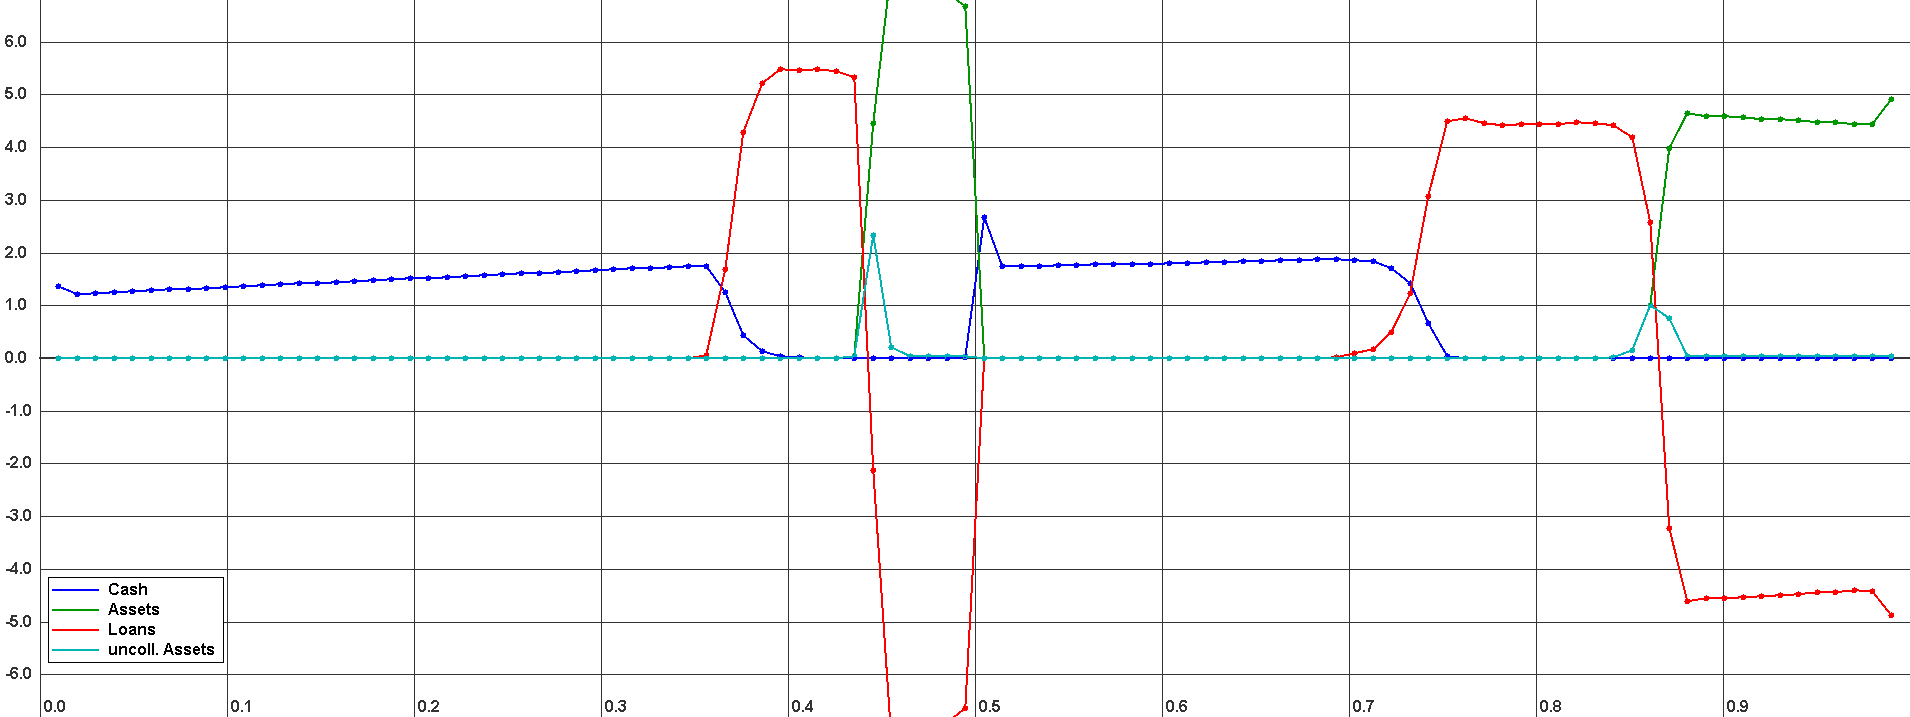
\includegraphics[width=1.0\textwidth, angle=0]{HALFFULLYCONNECTED_100_NOCOLLATERALMARKET_REPL.png}
	\caption{Wealth-Distribution of Half-Fully Connected topology }
	\label{fig:wealth_HALFFULLYCONNECTED_100_NOCOLLATERALMARKET_REPL}
\end{figure}

\begin{table}[H]
	\caption{Equilibrium of Half-Fully Connected topology}
	\centering
	\begin{tabular} { l c r }
		\hline
		Asset-price p & 0.526 (0.011) \\
		Bond-price q & 0.313 (0.003) \\
		Marginal agent i1 & 0.730 (0.011) \\
		Marginal agent i2 & 0.448 (0.005) \\
		\hline
		Pessimist wealth & 1.342 (0.022) \\
		Medianist wealth & 4.542 (0.353) \\
		Optimist wealth & 1.746 (0.074) \\
		\hline
	\end{tabular}
\end{table} 

\begin{table}[H]
	\caption{Performance of Half-Fully Connected topology}
	\centering
	\begin{tabular} { l c r }
		\hline
		Successful matching-rounds & 16,373.48 (493.96) \\
		Failed matching-rounds & 1,000.00 (0.00) \\
		Total matching-rounds & 17,373.48 (493.96) \\
		\hline
		Ratio successful/total & 0.94 \\
		Ratio failed/total & 0.06 \\
		\hline
	\end{tabular}
\end{table}

The equilibrium is clearly distinct from the theoretical and Fully-Connected one as miss-allocation can be found within the pessimists-range. Also the i1- and i2-points and the wealth-distributions differ both numerically and visually. 

\section{Ascending-Connected with short-cuts}
\label{app:results_acShortCuts}

\subsection{Random short-cuts}
\begin{figure}[H]
	\centering
  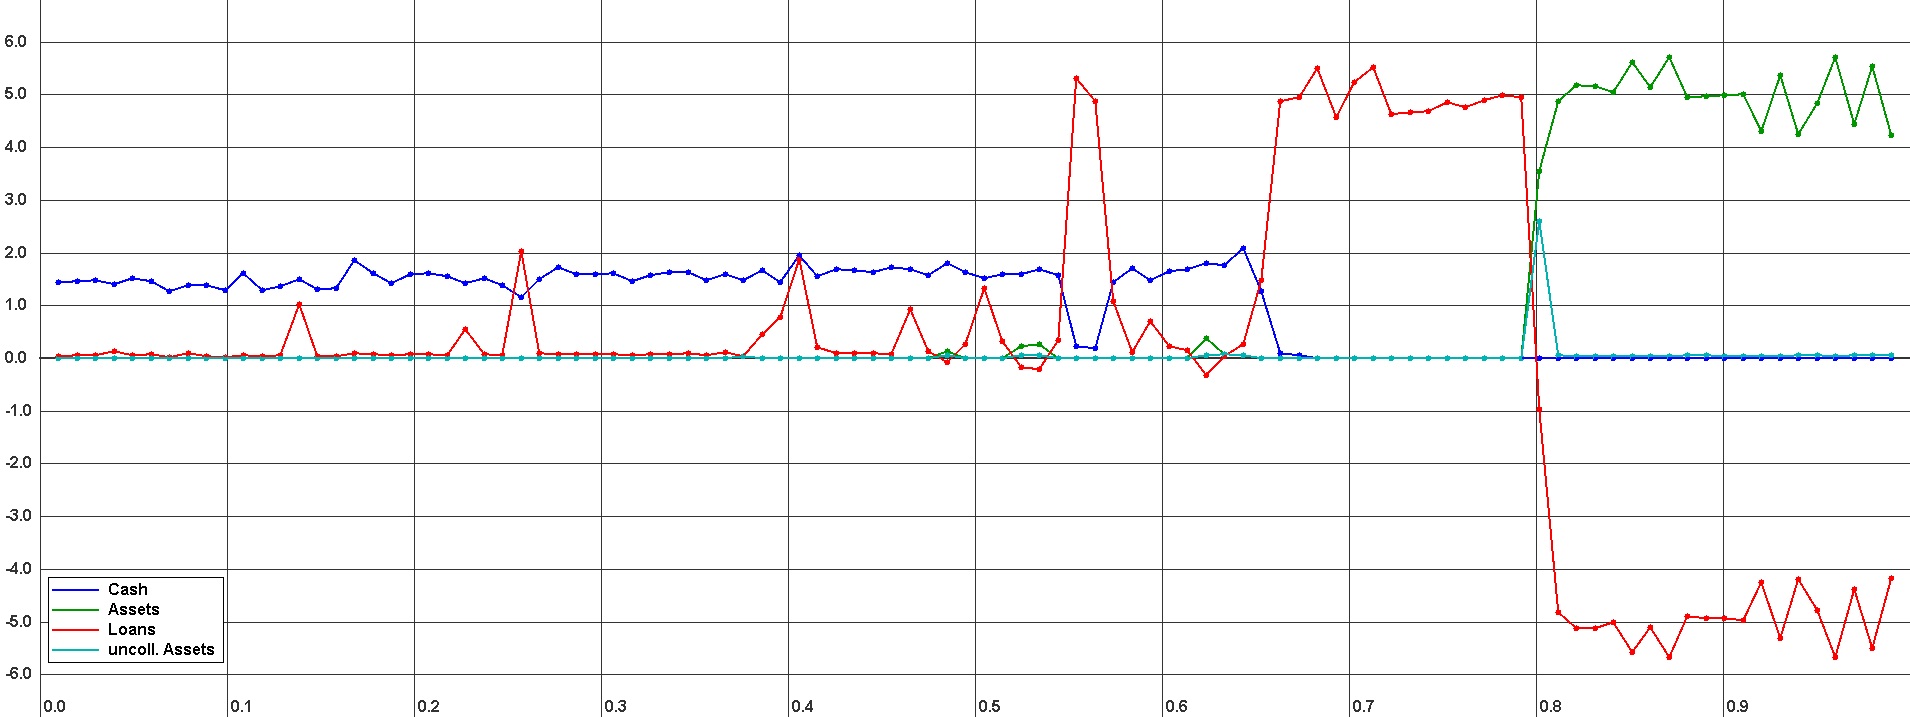
\includegraphics[width=1.0\textwidth, angle=0]{ASCENDINGCONNECTED_RANDSHORTCUTS_100_NOCOLLATERALMARKET_REPL.png}
	\caption{Wealth-Distribution of Ascending-Connected random short-cuts topology}
	\label{fig:wealth_ASCENDINGCONNECTED_RANDSHORTCUTS_100_NOCOLLATERALMARKET_REPL}
\end{figure}

\begin{table}[H]
	\caption{Equilibrium of Ascending-Connected random short-cuts topology}
	\centering
	\begin{tabular} { l c r }
		\hline
		Asset-price p & 0.704 (0.008) \\
		Bond-price q & 0.386 (0.003) \\
		Marginal agent i1 & 0.594 (0.000) \\
		Marginal agent i2 & 0.802 (0.000) \\
		\hline
		Pessimist wealth & 1.651 (0.003) \\
		Medianist wealth & 4.517 (0.428) \\
		Optimist wealth & 4.771 (0.249) \\
		\hline
	\end{tabular}
\end{table} 

\begin{table}[H]
	\caption{Performance of Ascending-Connected random short-cuts topology}
	\centering
	\begin{tabular} { l c r }
		\hline
		Successful matching-rounds & 7,249.40 (148.18) \\
		Failed matching-rounds & 1,000.60 (0.86) \\
		Total matching-rounds & 8,250.00 (148.21) \\
		\hline
		Ratio successful/total & 0.88 \\
		Ratio failed/total & 0.12 \\
		\hline
	\end{tabular}
\end{table}

Random short-cuts seem to reduce the miss-allocation of pessimists-wealth a bit but lead to a fundamental different equilibrium than the theoretical or fully-connected one as can clearly be seen both visually and numerically.

\subsection{2 short-cuts}
\begin{figure}[H]
	\centering
  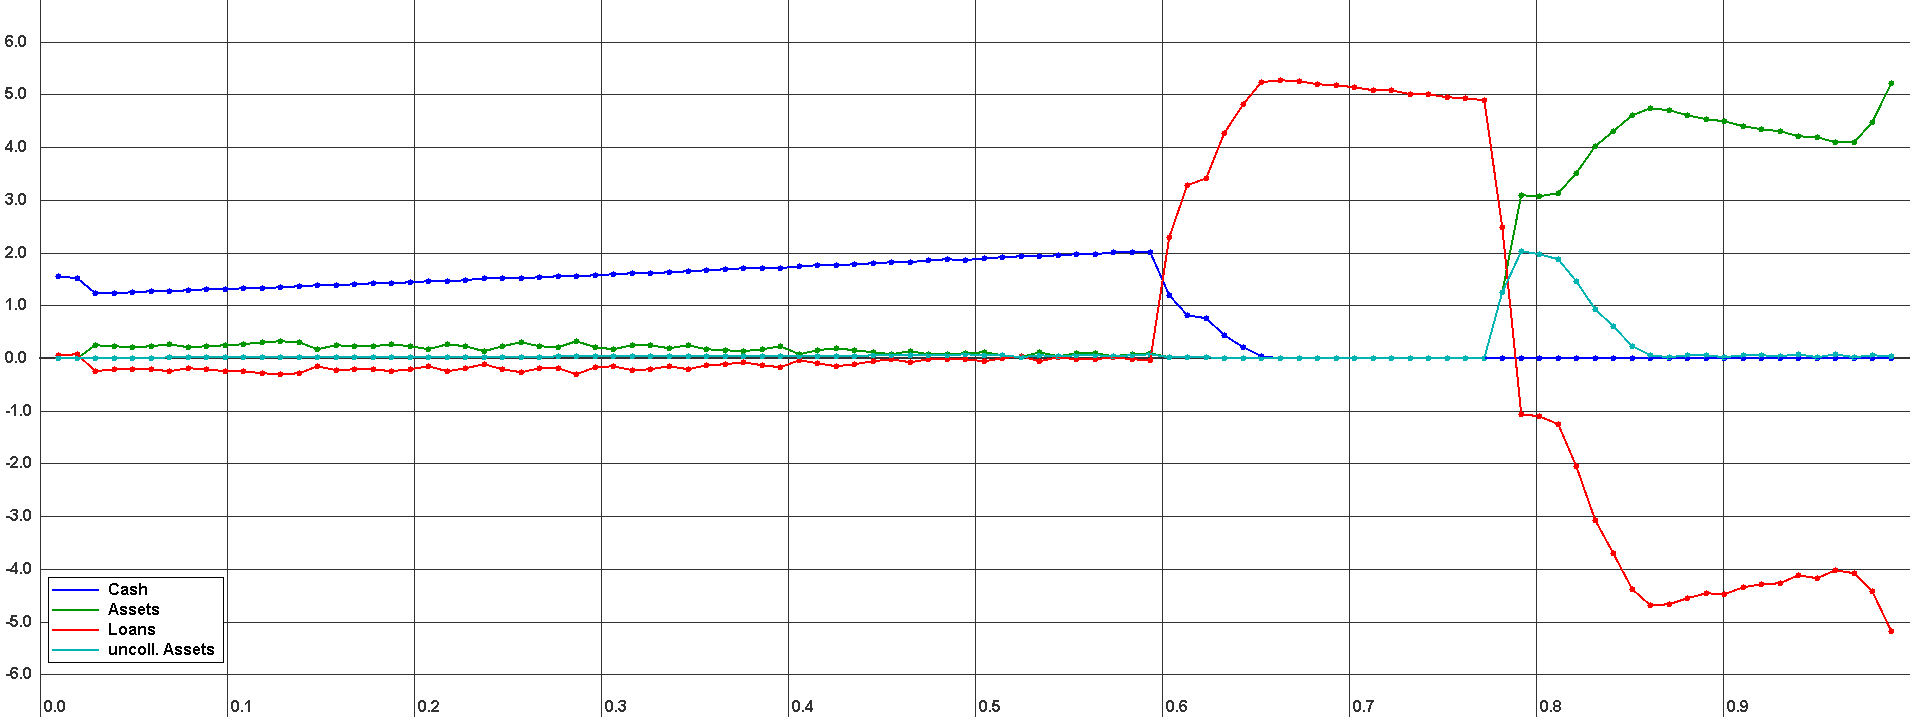
\includegraphics[width=1.0\textwidth, angle=0]{ASCENDINGCONNECTED_2SC_100_NOCOLLATERALMARKET_REPL.png}
	\caption{Wealth-Distribution of Ascending-Connected 2 short-cuts topology}
	\label{fig:wealth_ASCENDINGCONNECTED_2SC_100_NOCOLLATERALMARKET_REPL}
\end{figure}

\begin{table}[H]
	\caption{Equilibrium of Ascending-Connected 2 short-cuts topology}
	\centering
	\begin{tabular} { l c r }
		\hline
		Asset-price p & 0.706 (0.010) \\
		Bond-price q & 0.379 (0.001) \\
		Marginal agent i1 & 0.592 (0.004) \\
		Marginal agent i2 & 0.782 (0.001) \\
		\hline
		Pessimist wealth & 1.667 (0.001) \\
		Medianist wealth & 5.207 (0.105) \\
		Optimist wealth & 4.544 (0.039) \\
		\hline
	\end{tabular}
\end{table} 

\begin{table}[H]
	\caption{Performance of Ascending-Connected random short-cuts topology}
	\centering
	\begin{tabular} { l c r }
		\hline
		Successful matching-rounds & 26,572.90 (91.85) \\
		Failed matching-rounds & 1,000.64 (1.03) \\
		Total matching-rounds & 27,573.54 (91.99) \\
		\hline
		Ratio successful/total & 0.96 \\
		Ratio failed/total & 0.04 \\
		\hline
	\end{tabular}
\end{table}

This topology reduces the miss-allocation in the pessimists-range dramatically but doesn't solve it yet. Unfortunately it leads to a dramatically different wealth-distribution within the medianists and optimist.

\subsection{5 full short-cuts}
\begin{figure}[H]
	\centering
  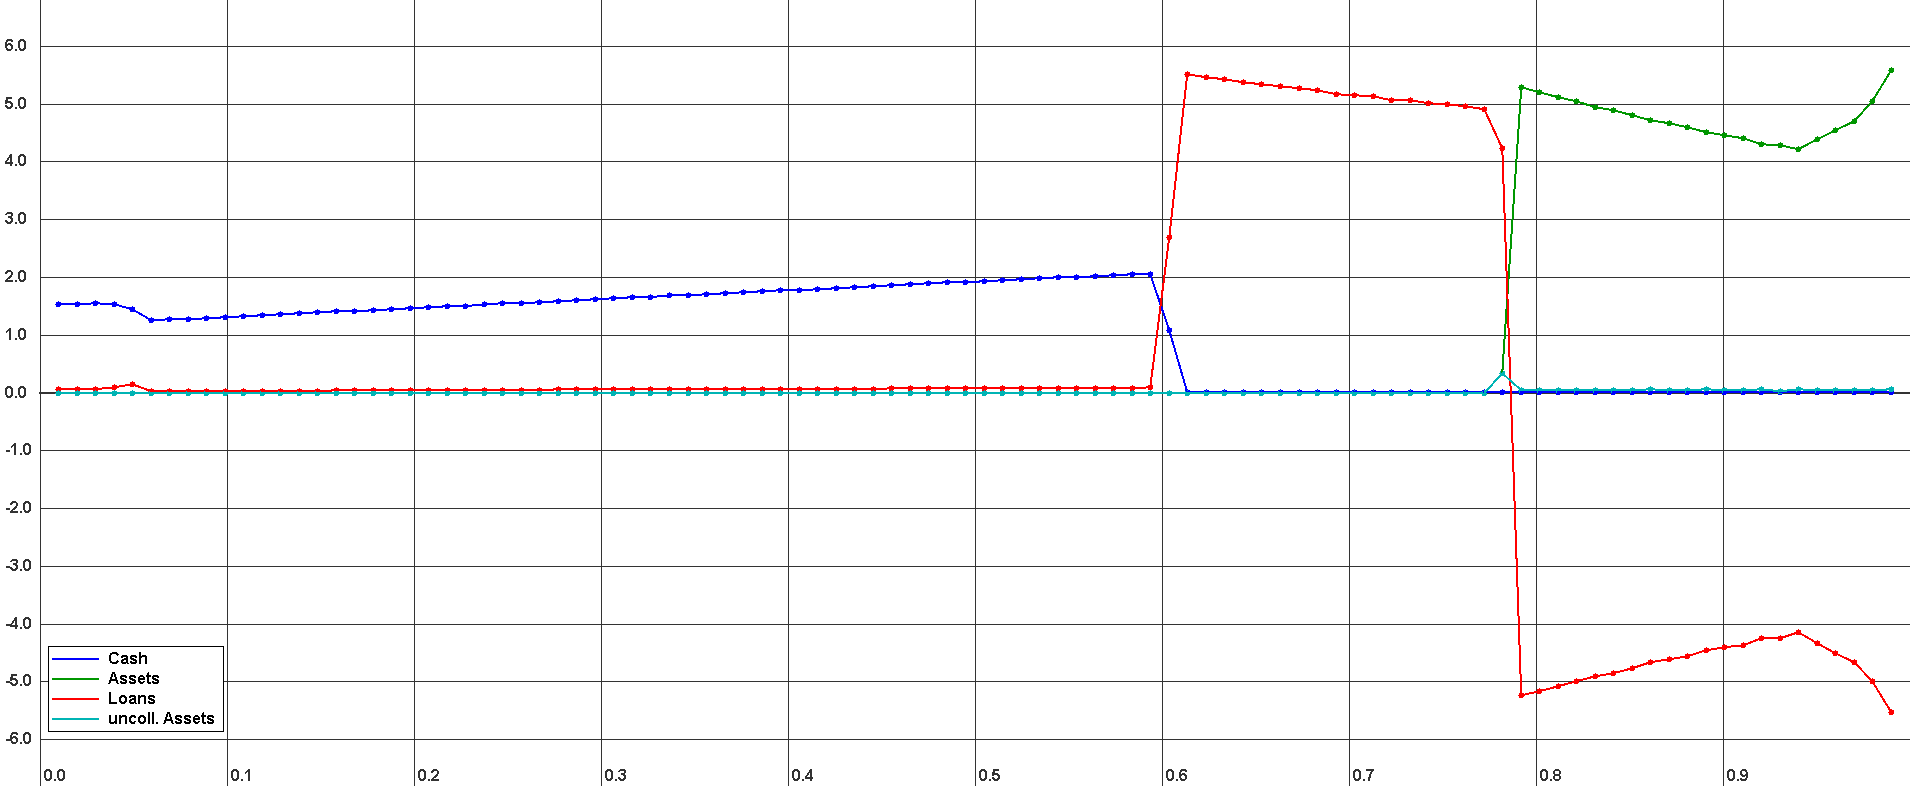
\includegraphics[width=1.0\textwidth, angle=0]{ASCENDINGCONNECTED_5FullSC_100_NOCOLLATERALMARKET_REPL.png}
	\caption{Wealth-Distribution of Ascending-Connected 5 full short-cuts topology}
	\label{fig:wealth_ASCENDINGCONNECTED_5FullSC_100_NOCOLLATERALMARKET_REPL}
\end{figure}

\begin{table}[H]
	\caption{Equilibrium of Ascending-Connected 5 full short-cuts}
	\centering
	\begin{tabular} { l c r }
		\hline
		Asset-price p & 0.692 (0.010) \\
		Bond-price q & 0.379 (0.001) \\
		Marginal agent i1 & 0.594 (0.000) \\
		Marginal agent i2 & 0.792 (0.000) \\
		\hline
		Pessimist wealth & 1.667 (0.000) \\
		Medianist wealth & 5.160 (0.026) \\
		Optimist wealth & 4.747 (0.013) \\
		\hline
	\end{tabular}
\end{table} 

\begin{table}[H]
	\caption{Performance of Ascending-Connected 5 full short-cuts topology}
	\centering
	\begin{tabular} { l c r }
		\hline
		Successful matching-rounds & 11,157.56 (79.45) \\
		Failed matching-rounds & 1,000.92 (1.08) \\
		Total matching-rounds & 12,158.48 (79.36) \\
		\hline
		Ratio successful/total & 0.92 \\
		Ratio failed/total & 0.08 \\
		\hline
	\end{tabular}
\end{table}

As can be clearly seen this topology seems to be able to solve miss-allocations in the pessimists-range seen in Ascending-Connected topology but is still different than the theoretical and Fully-Connected equilibrium.

\subsection{15 full short-cuts}
\begin{figure}[H]
	\centering
  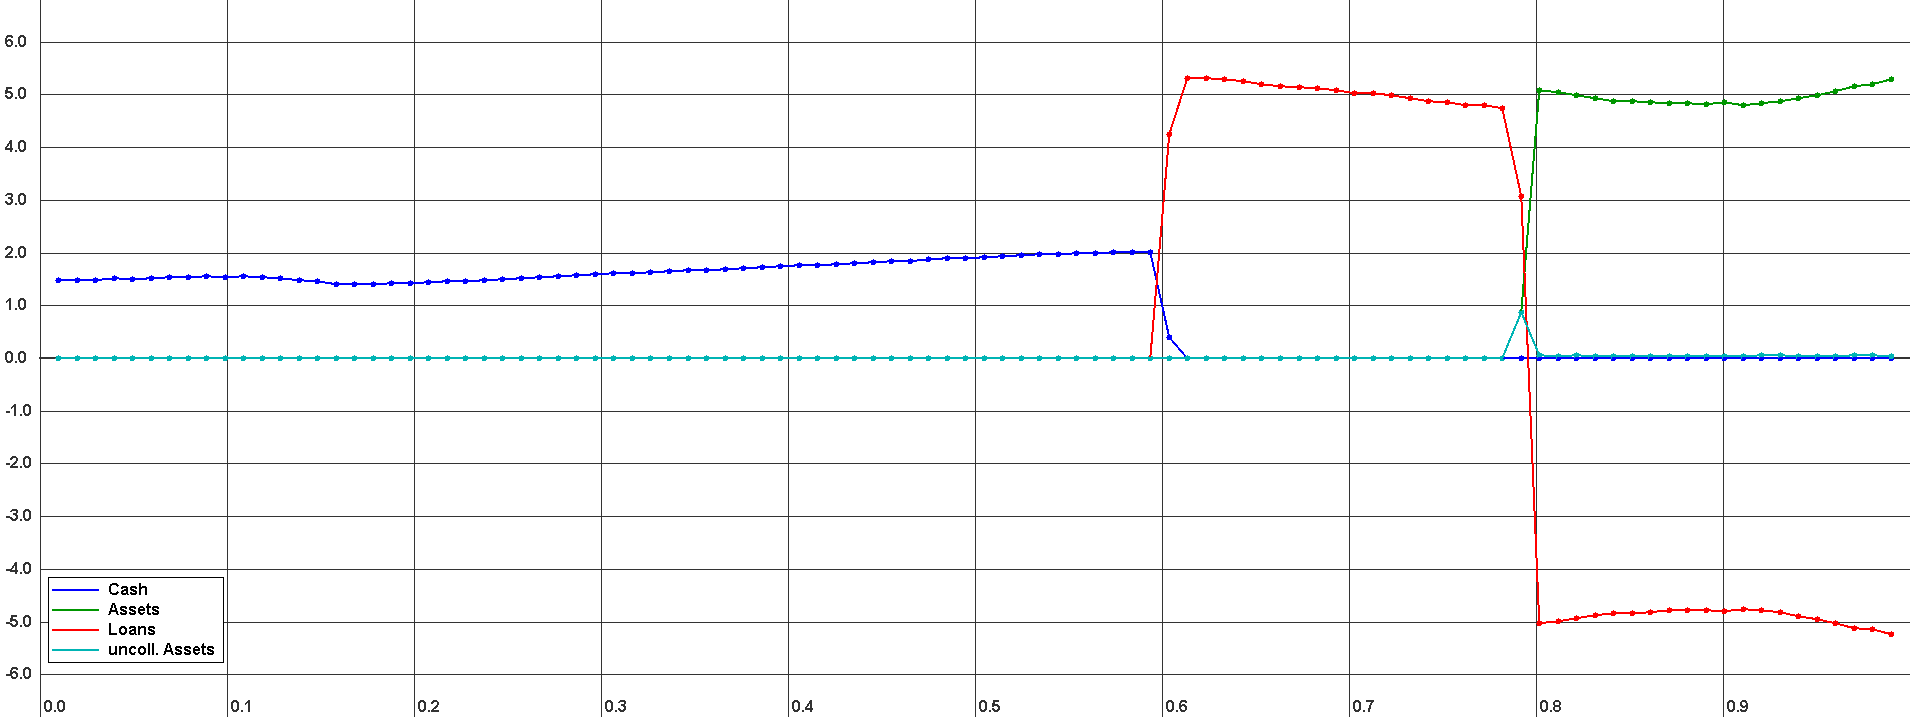
\includegraphics[width=1.0\textwidth, angle=0]{ASCENDINGCONNECTED_15FullSC_100_NOCOLLATERALMARKET_REPL.png}
	\caption{Wealth-Distribution of Ascending-Connected 15 full short-cuts topology}
	\label{fig:wealth_ASCENDINGCONNECTED_15FullSC_100_NOCOLLATERALMARKET_REPL}
\end{figure}

\begin{table}[H]
	\caption{Equilibrium of Ascending-Connected 15 full short-cuts topology}
	\centering
	\begin{tabular} { l c r }
		\hline
		Asset-price p & 0.687 (0.012) \\
		Bond-price q & 0.380 (0.001) \\
		Marginal agent i1 & 0.594 (0.000) \\
		Marginal agent i2 & 0.801 (0.002) \\
		\hline
		Pessimist wealth & 1.660 (0.003) \\
		Medianist wealth & 4.922 (0.039) \\
		Optimist wealth & 4.948 (0.052) \\
		\hline
	\end{tabular}
\end{table} 

\begin{table}[H]
	\caption{Performance of Ascending-Connected 15 full short-cuts topology}
	\centering
	\begin{tabular} { l c r }
		\hline
		Successful matching-rounds & 3,716.52 (42.31) \\
		Failed matching-rounds & 1,000.66 (0.98) \\
		Total matching-rounds & 4,717.18 (42.18) \\
		\hline
		Ratio successful/total & 0.79 \\
		Ratio failed/total & 0.21 \\
		\hline
	\end{tabular}
\end{table}

This topology comes very close to the theoretical equilibrium but is still a bit different as can be seen in the curved wealth-distributions of the pure optimists.

\subsection{30 full short-cuts}
\begin{figure}[H]
	\centering
  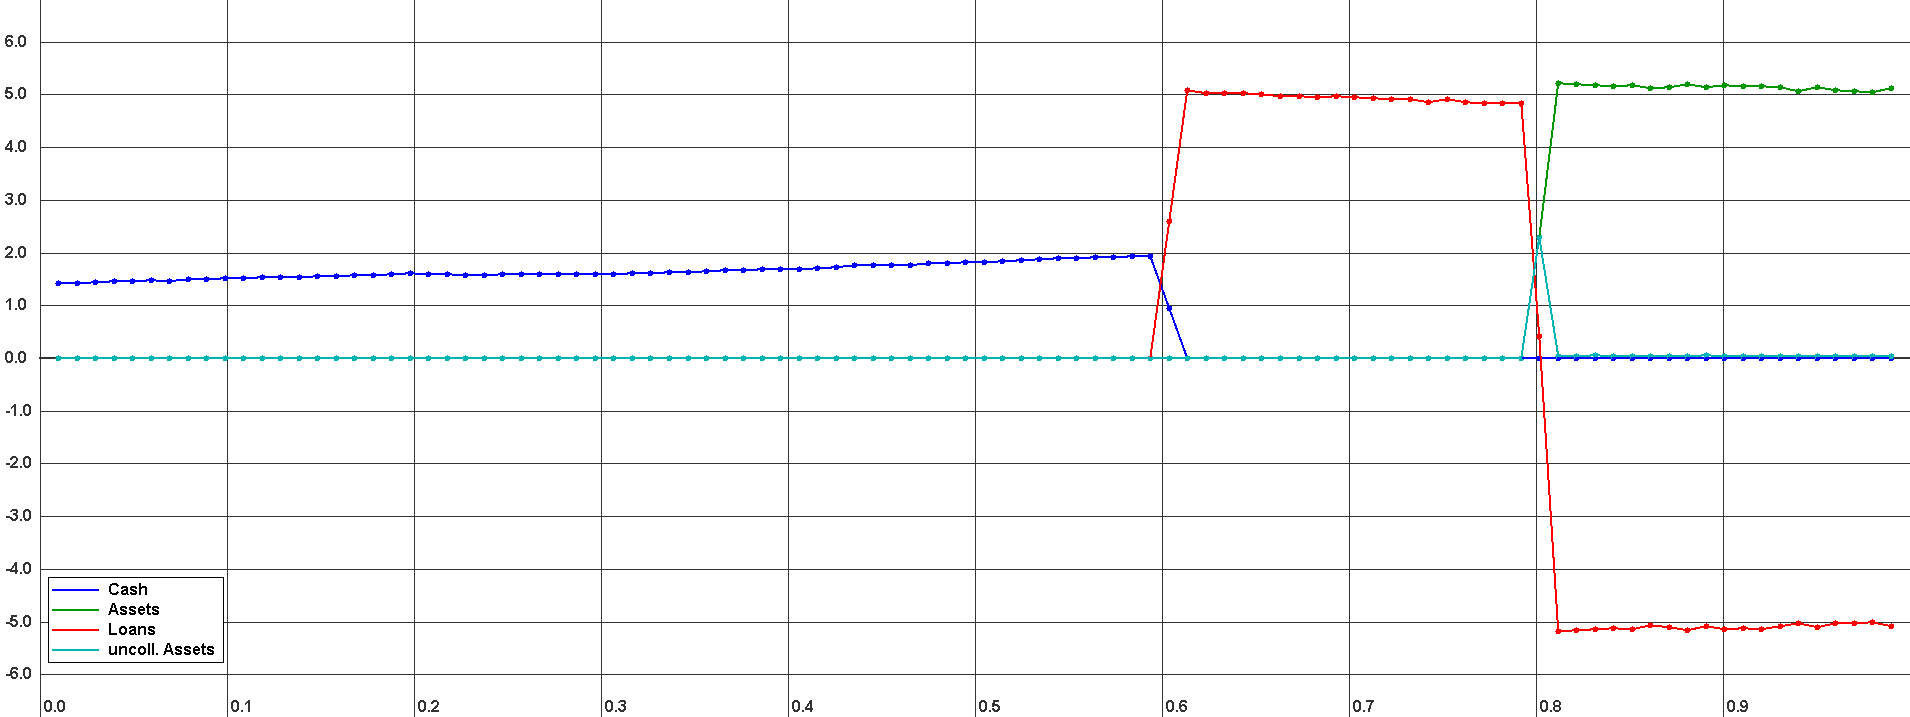
\includegraphics[width=1.0\textwidth, angle=0]{ASCENDINGCONNECTED_30FullSC_100_NOCOLLATERALMARKET_REPL.png}
	\caption{Wealth-Distribution of Ascending-Connected 30 full short-cuts topology}
	\label{fig:wealth_ASCENDINGCONNECTED_30FullSC_100_NOCOLLATERALMARKET_REPL}
\end{figure}

\begin{table}[H]
	\caption{Equilibrium of Ascending-Connected 30 full short-cuts topology}
	\centering
	\begin{tabular} { l c r }
		\hline
		Asset-price p & 0.705 (0.015) \\
		Bond-price q & 0.382 (0.001) \\
		Marginal agent i1 & 0.594 (0.001) \\
		Marginal agent i2 & 0.803 (0.003) \\
		\hline
		Pessimist wealth & 1.651 (0.004) \\
		Medianist wealth & 4.812 (0.062) \\
		Optimist wealth & 5.027 (0.068) \\
		\hline
	\end{tabular}
\end{table} 

\begin{table}[H]
	\caption{Performance of Ascending-Connected 30 full short-cuts topology}
	\centering
	\begin{tabular} { l c r }
		\hline
		Successful matching-rounds & 2,062.92 (28.59) \\
		Failed matching-rounds & 1,000.42 (0.78) \\
		Total matching-rounds & 3,063.34 (28.49) \\
		\hline
		Ratio successful/total & 0.67 \\
		Ratio failed/total & 0.33 \\
		\hline
	\end{tabular}
\end{table}

This topology is very close to the theoretical and Fully-Connected equilibrium although it differs in asset-price p and in the wealth-distributions. Of course with 30 fully short-cuts in a network of 100 agents one is already very close to fully connectedness.

\subsection{5 regular short-cuts}
\begin{figure}[H]
	\centering
  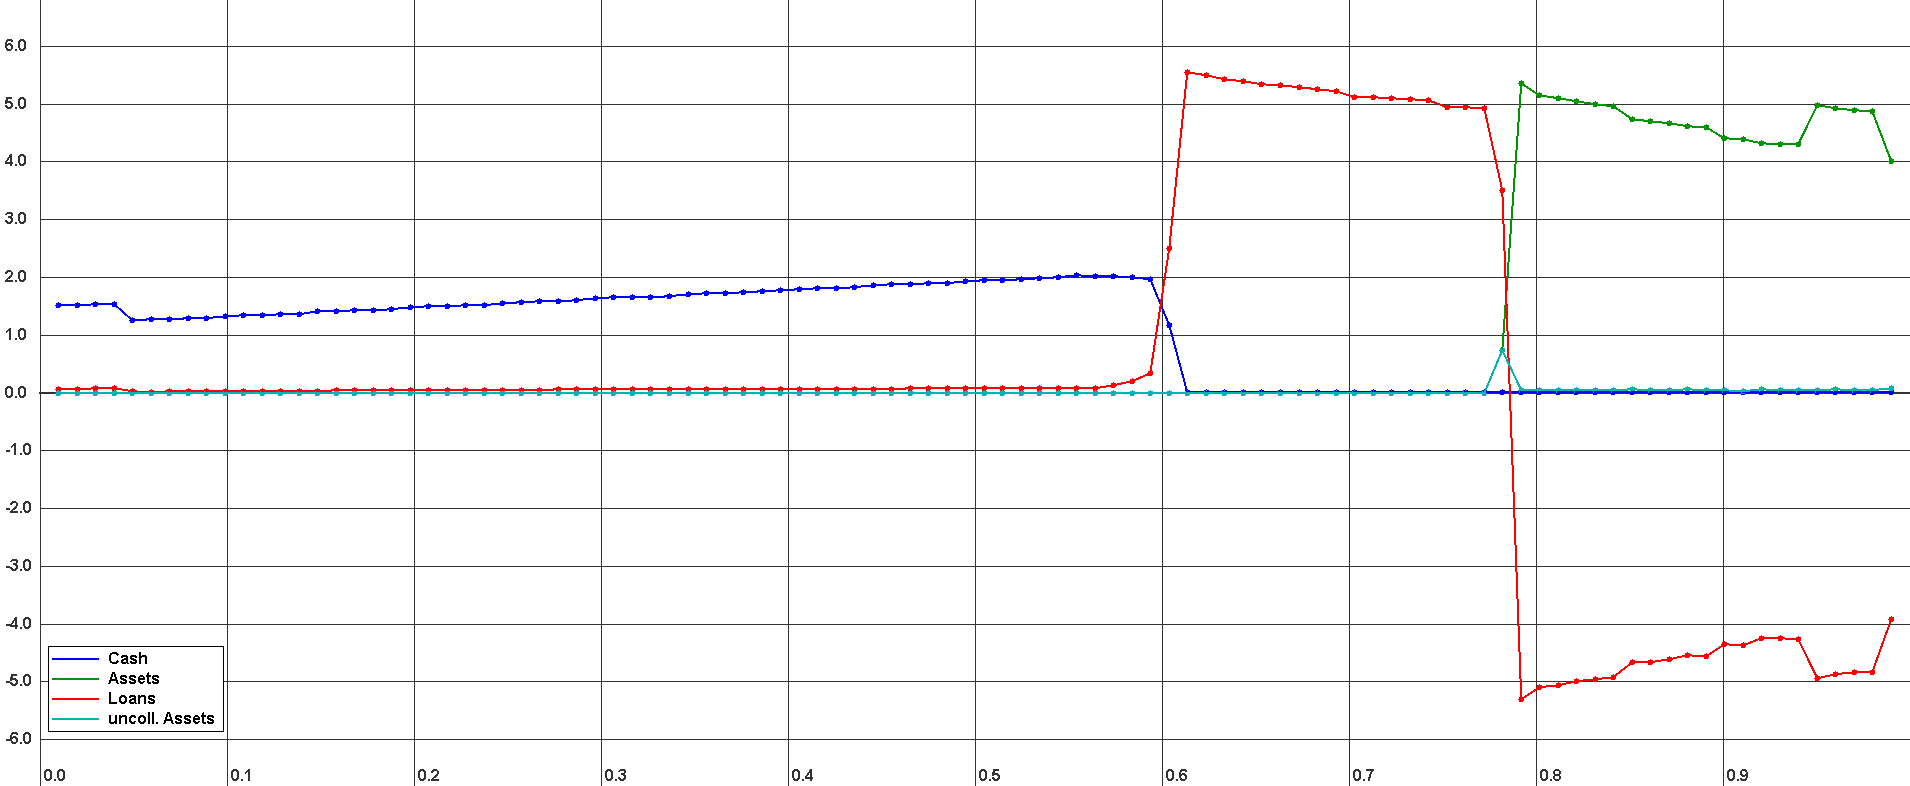
\includegraphics[width=1.0\textwidth, angle=0]{ASCENDINGCONNECTED_5RegSC_100_NOCOLLATERALMARKET_REPL.png}
	\caption{Wealth-Distribution of Ascending-Connected 5 regular short-cuts topology}
	\label{fig:wealth_ASCENDINGCONNECTED_5RegSC_100_NOCOLLATERALMARKET_REPL}
\end{figure}

\begin{table}[H]
	\caption{Equilibrium of Ascending-Connected 5 regular short-cuts topology}
	\centering
	\begin{tabular} { l c r }
		\hline
		Asset-price p & 0.694 (0.013) \\
		Bond-price q & 0.379 (0.002) \\
		Marginal agent i1 & 0.594 (0.000) \\
		Marginal agent i2 & 0.792 (0.000) \\
		\hline
		Pessimist wealth & 1.667 (0.000) \\
		Medianist wealth & 5.130 (0.029) \\
		Optimist wealth & 4.726 (0.014) \\
		\hline
	\end{tabular}
\end{table} 

\begin{table}[H]
	\caption{Performance of Ascending-Connected 5 regular short-cuts topology}
	\centering
	\begin{tabular} { l c r }
		\hline
		Successful matching-rounds & 9,743.36 (52.60) \\
		Failed matching-rounds & 1,000.64 (0.69) \\
		Total matching-rounds & 10,744.00 (52.72) \\
		\hline
		Ratio successful/total & 0.91 \\
		Ratio failed/total & 0.09 \\
		\hline
	\end{tabular}
\end{table}

As can be seen in the visual results this topology shows a different equilibrium than the theoretical and Fully-Connected one.

\subsection{15 regular short-cuts}
\begin{figure}[H]
	\centering
  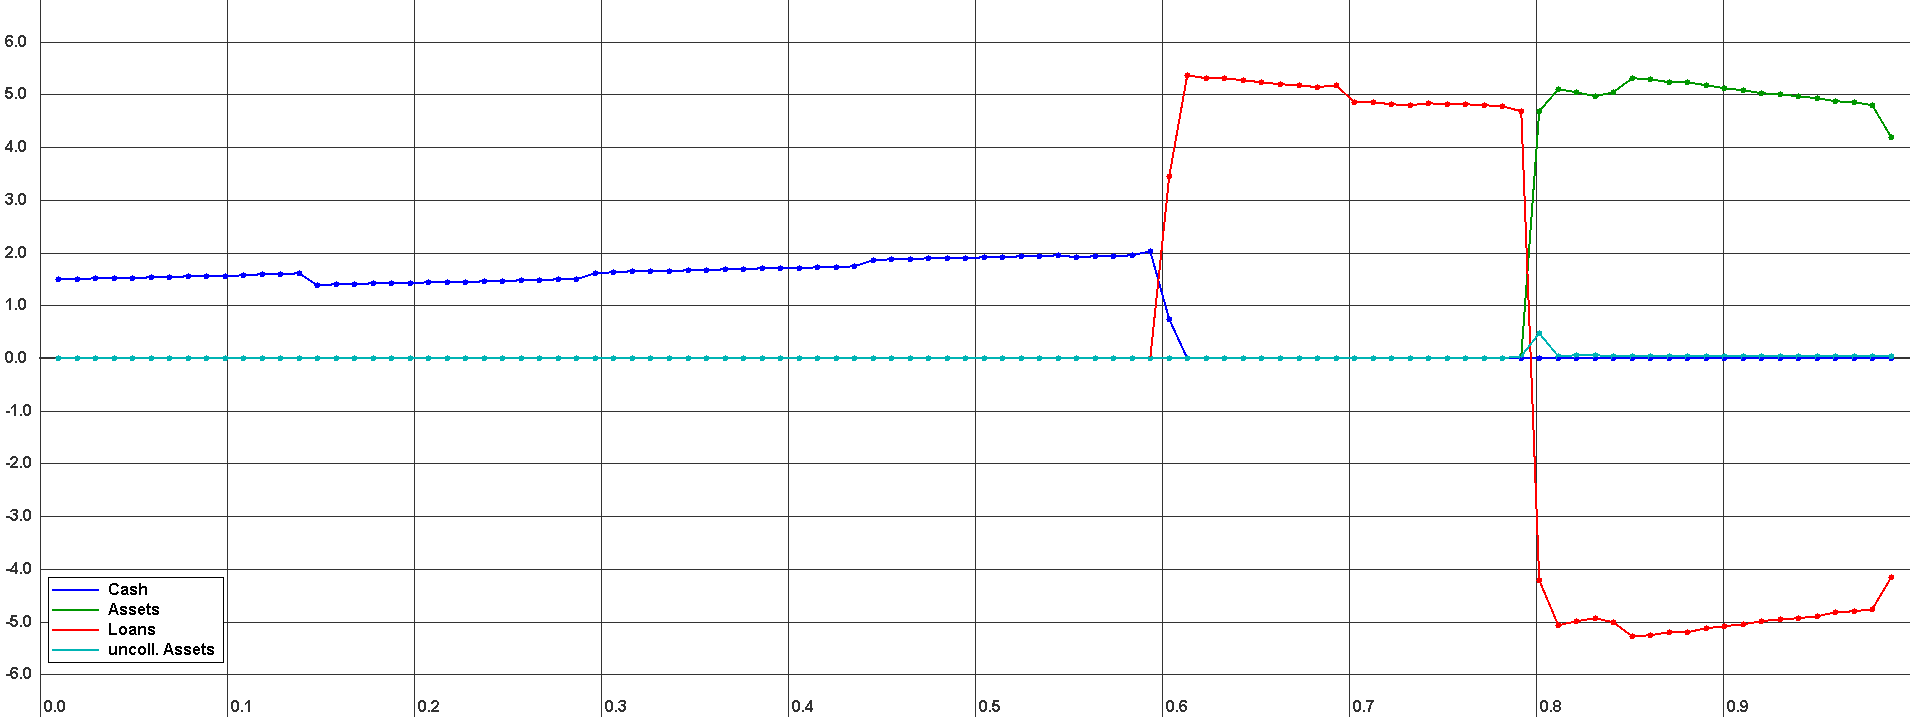
\includegraphics[width=1.0\textwidth, angle=0]{ASCENDINGCONNECTED_15RegSC_100_NOCOLLATERALMARKET_REPL.png}
	\caption{Wealth-Distribution of Ascending-Connected 15 regular short-cuts topology}
	\label{fig:wealth_ASCENDINGCONNECTED_15RegSC_100_NOCOLLATERALMARKET_REPL}
\end{figure}

\begin{table}[H]
	\caption{Equilibrium Ascending-Connected 15 regular short-cuts topology}
	\centering
	\begin{tabular} { l c r }
		\hline
		Asset-price p & 0.678 (0.018) \\
		Bond-price q & 0.382 (0.001) \\
		Marginal agent i1 & 0.594 (0.000) \\
		Marginal agent i2 & 0.802 (0.000) \\
		\hline
		Pessimist wealth & 1.654 (0.002) \\
		Medianist wealth & 4.933 (0.014) \\
		Optimist wealth & 4.998 (0.005) \\
		\hline
	\end{tabular}
\end{table} 

\begin{table}[H]
	\caption{Performance of Ascending-Connected 15 regular short-cuts topology}
	\centering
	\begin{tabular} { l c r }
		\hline
		Successful matching-rounds & 4,090.94 (51.71) \\
		Failed matching-rounds & 1,007.40 (38.50) \\
		Total matching-rounds & 5,098.34 (73.30) \\
		\hline
		Ratio successful/total & 0.80 \\
		Ratio failed/total & 0.20 \\
		\hline
	\end{tabular}
\end{table}

The equilibrium of this topology is falls very far from the theoretical and Fully-Connected one.

\subsection{30 regular short-cuts}
\begin{figure}[H]
	\centering
  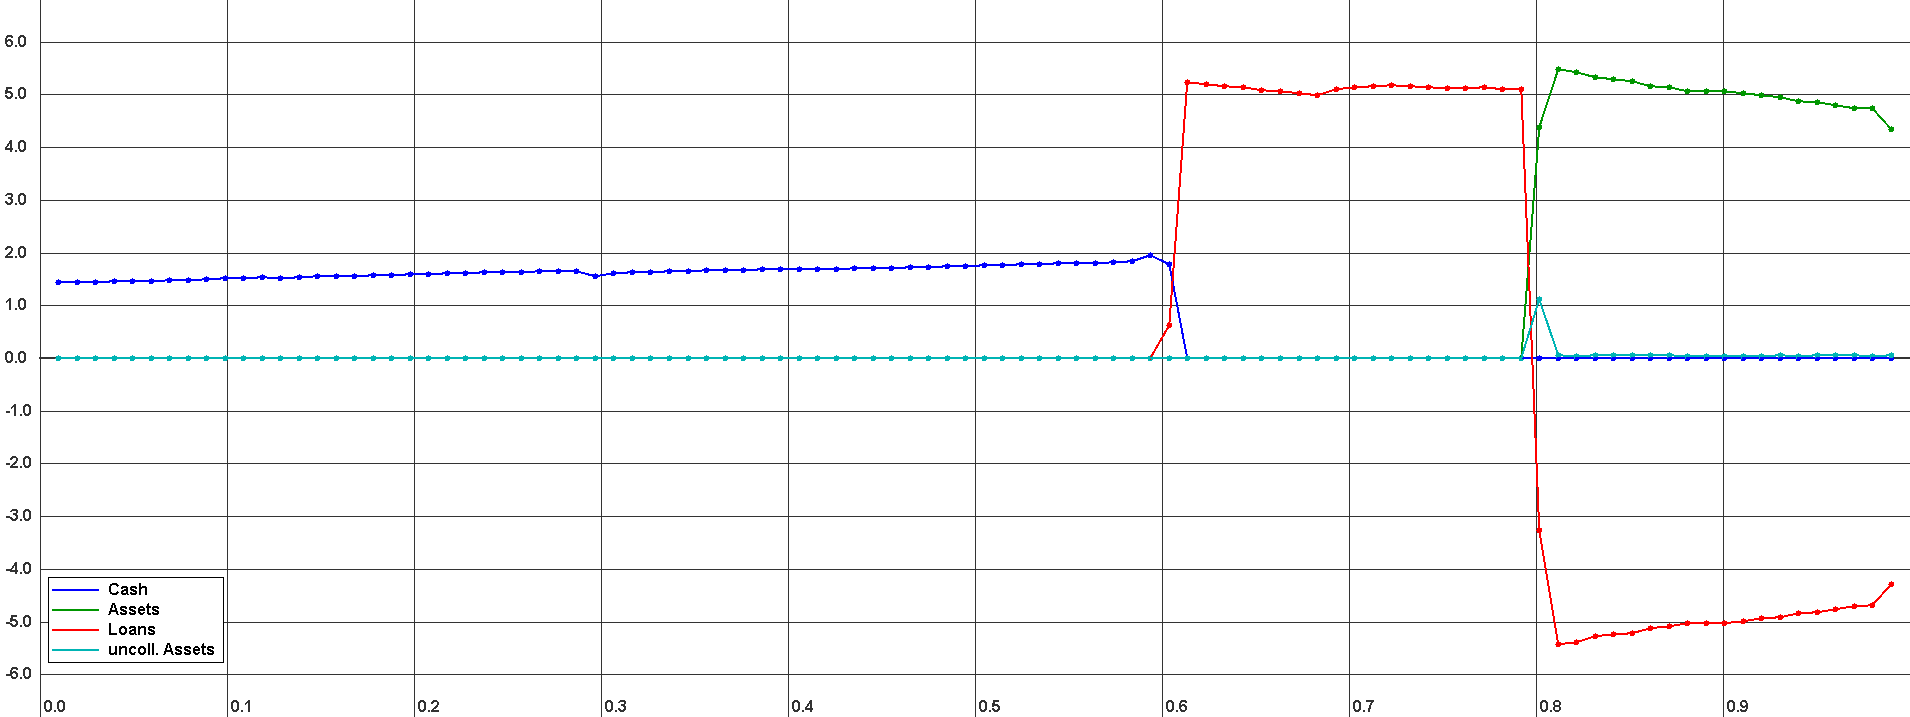
\includegraphics[width=1.0\textwidth, angle=0]{ASCENDINGCONNECTED_30RegSC_100_NOCOLLATERALMARKET_REPL.png}
	\caption{Wealth-Distribution of Ascending-Connected 30 regular short-cuts topology}
	\label{fig:wealth_ASCENDINGCONNECTED_30RegSC_100_NOCOLLATERALMARKET_REPL}
\end{figure}

\begin{table}[H]
	\caption{Equilibrium of Ascending-Connected 30 regular short-cuts topology}
	\centering
	\begin{tabular} { l c r }
		\hline
		Asset-price p & 0.653 (0.045) \\
		Bond-price q & 0.382 (0.001) \\
		Marginal agent i1 & 0.604 (0.001) \\
		Marginal agent i2 & 0.802 (0.000) \\
		\hline
		Pessimist wealth & 1.639 (0.001) \\
		Medianist wealth & 5.120 (0.034) \\
		Optimist wealth & 5.000 (0.000) \\
		\hline
	\end{tabular}
\end{table} 

\begin{table}[H]
	\caption{Performance of Ascending-Connected 30 regular short-cuts topology}
	\centering
	\begin{tabular} { l c r }
		\hline
		Successful matching-rounds & 6,301.60 (162.67) \\
		Failed matching-rounds & 1,001.26 (1.38) \\
		Total matching-rounds & 7,302.86 (162.94) \\
		\hline
		Ratio successful/total & 0.86 \\
		Ratio failed/total & 0.14 \\
		\hline
	\end{tabular}
\end{table}

The equilibrium of this topology is falls very far from the theoretical and Fully-Connected one.

\section{Hub-Based topologies} 
The Hub-Based Topologies fail to come even close to equilibrium due to reasons given in chapter \ref{ch:hypothesis} "Hypothesis". This can be seen also very clearly in the visual results and thus no performance- and equilibrium-tables are listed as they would not make any sense.

\subsection{3-Hubs}
\begin{figure}[H]
	\centering
  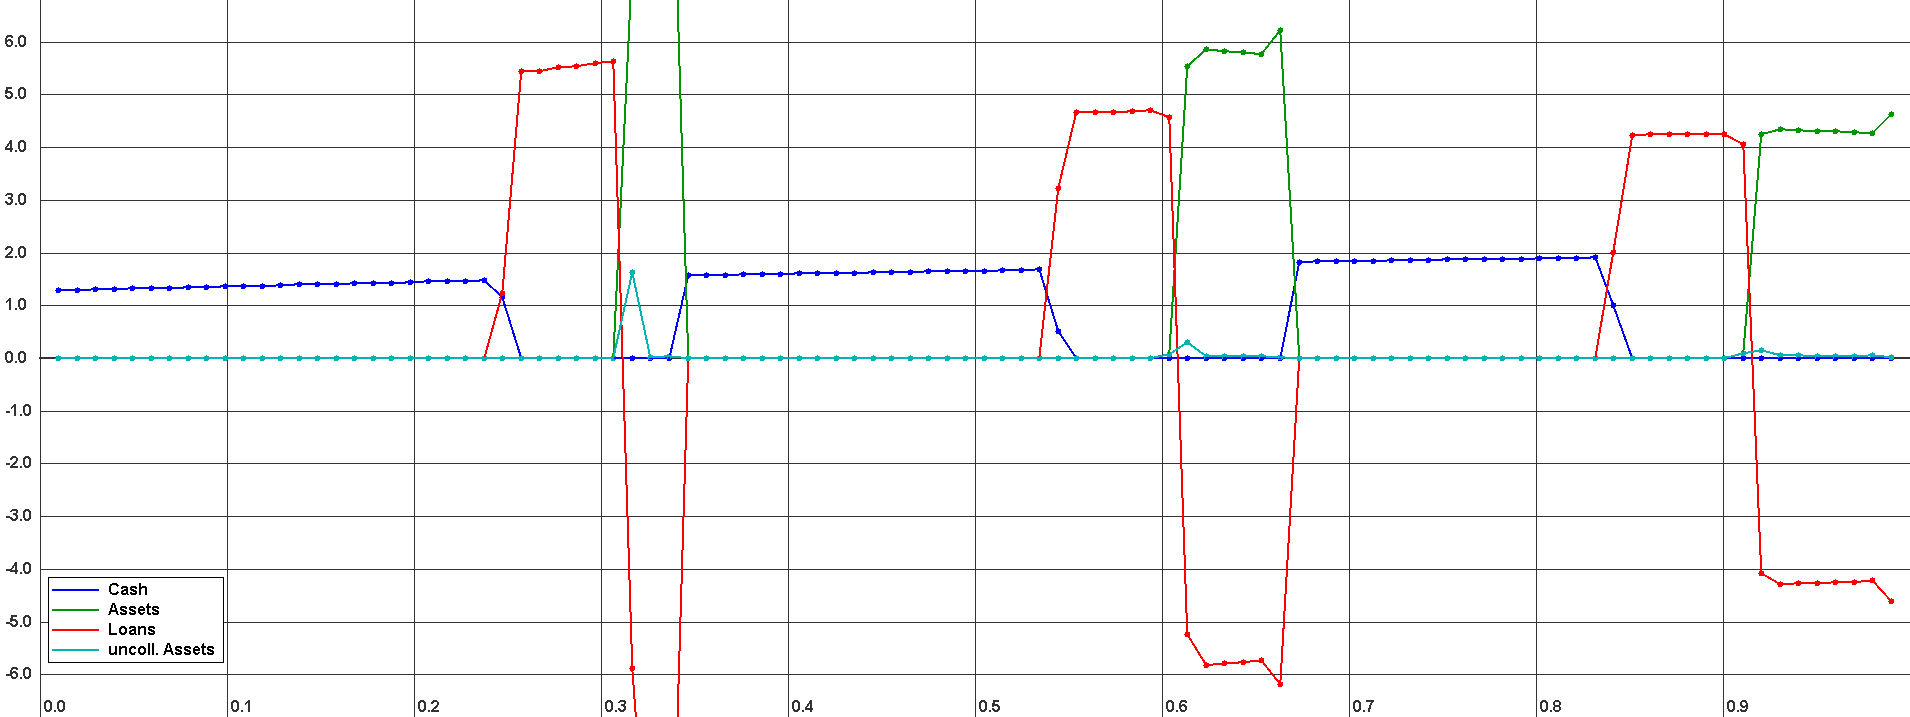
\includegraphics[width=1.0\textwidth, angle=0]{3HUBS_100_NOCOLLATERALMARKET_REPL.png}
	\caption{Wealth-Distribution of 3-Hubs topology}
	\label{fig:wealth_3HUBS_100_NOCOLLATERALMARKET_REPL}
\end{figure}

\subsection{1-Median Hub}
\begin{figure}[H]
	\centering
  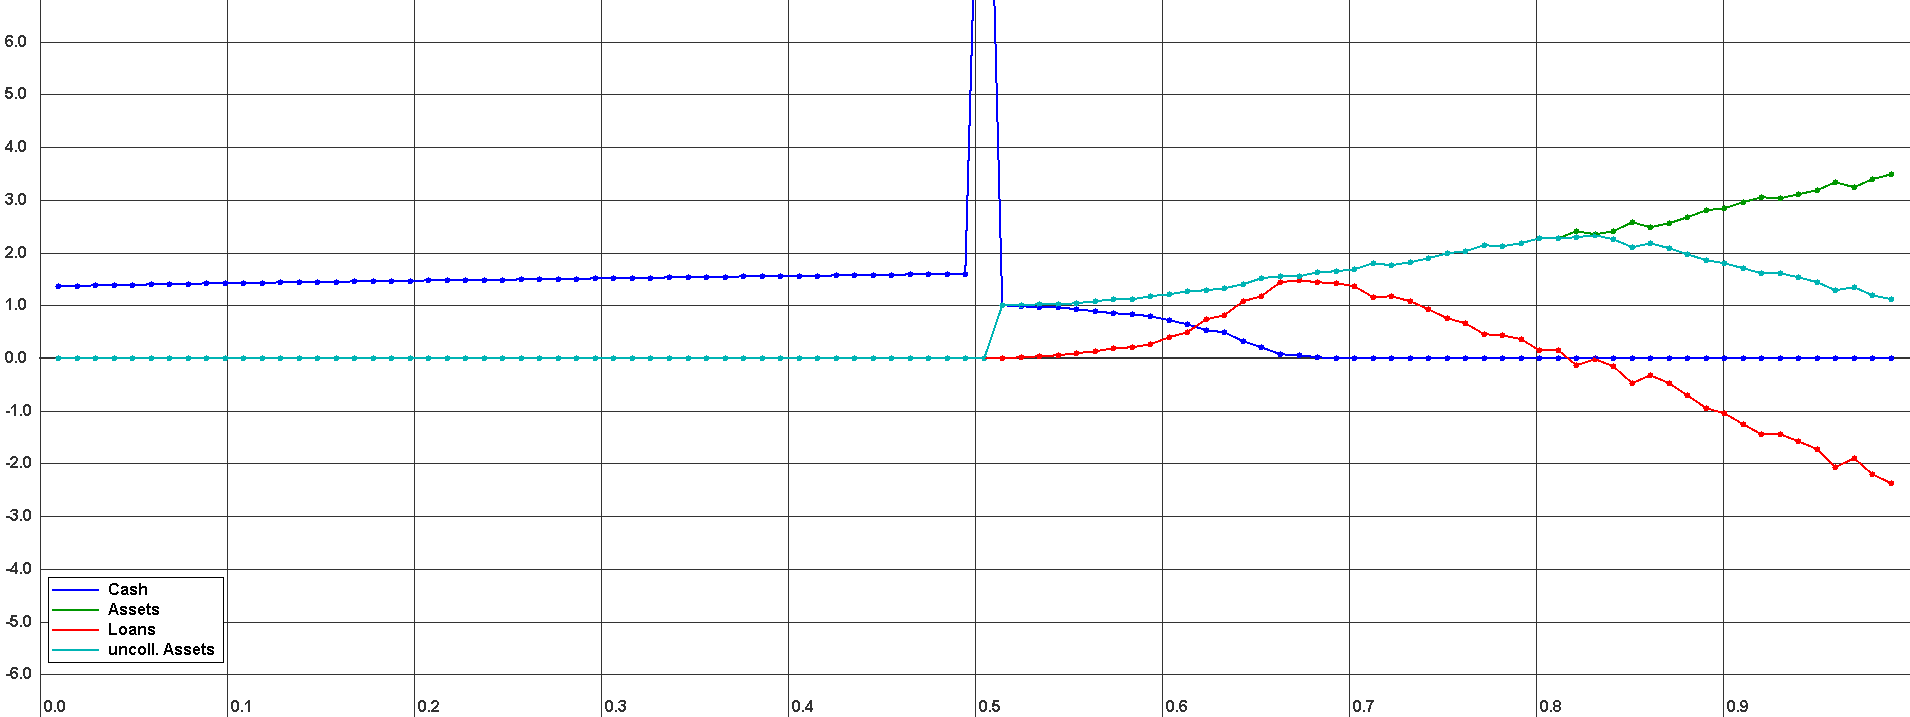
\includegraphics[width=1.0\textwidth, angle=0]{1MEDIANHUB_100_NOCOLLATERALMARKET_REPL.png}
	\caption{Wealth-Distribution of 1 Median-Hub topology}
	\label{fig:wealth_1MEDIANHUB_100_NOCOLLATERALMARKET_REPL}
\end{figure}

\subsection{3-Median Hubs}
\begin{figure}[H]
	\centering
  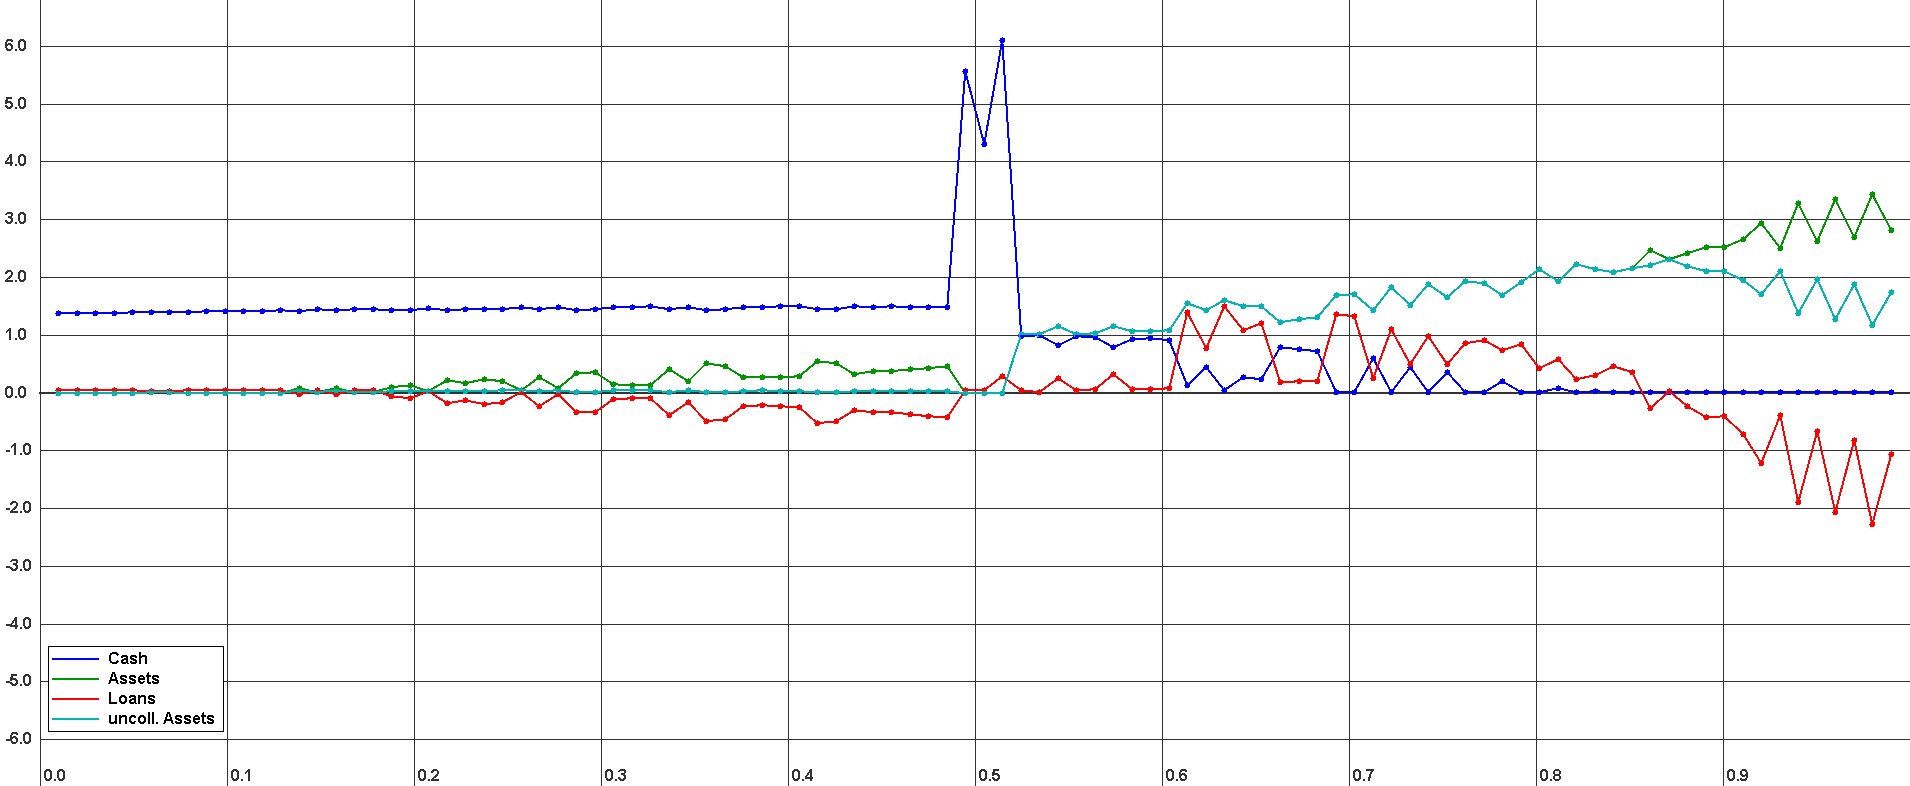
\includegraphics[width=1.0\textwidth, angle=0]{3MEDIANHUBS_100_NOCOLLATERALMARKET_REPL.png}
	\caption{Wealth-Distribution of 3 Median-Hubs topology}
	\label{fig:wealth_3MEDIANHUBS_100_NOCOLLATERALMARKET_REPL}
\end{figure}

\subsection{Maximum Hub}
\begin{figure}[H]
	\centering
  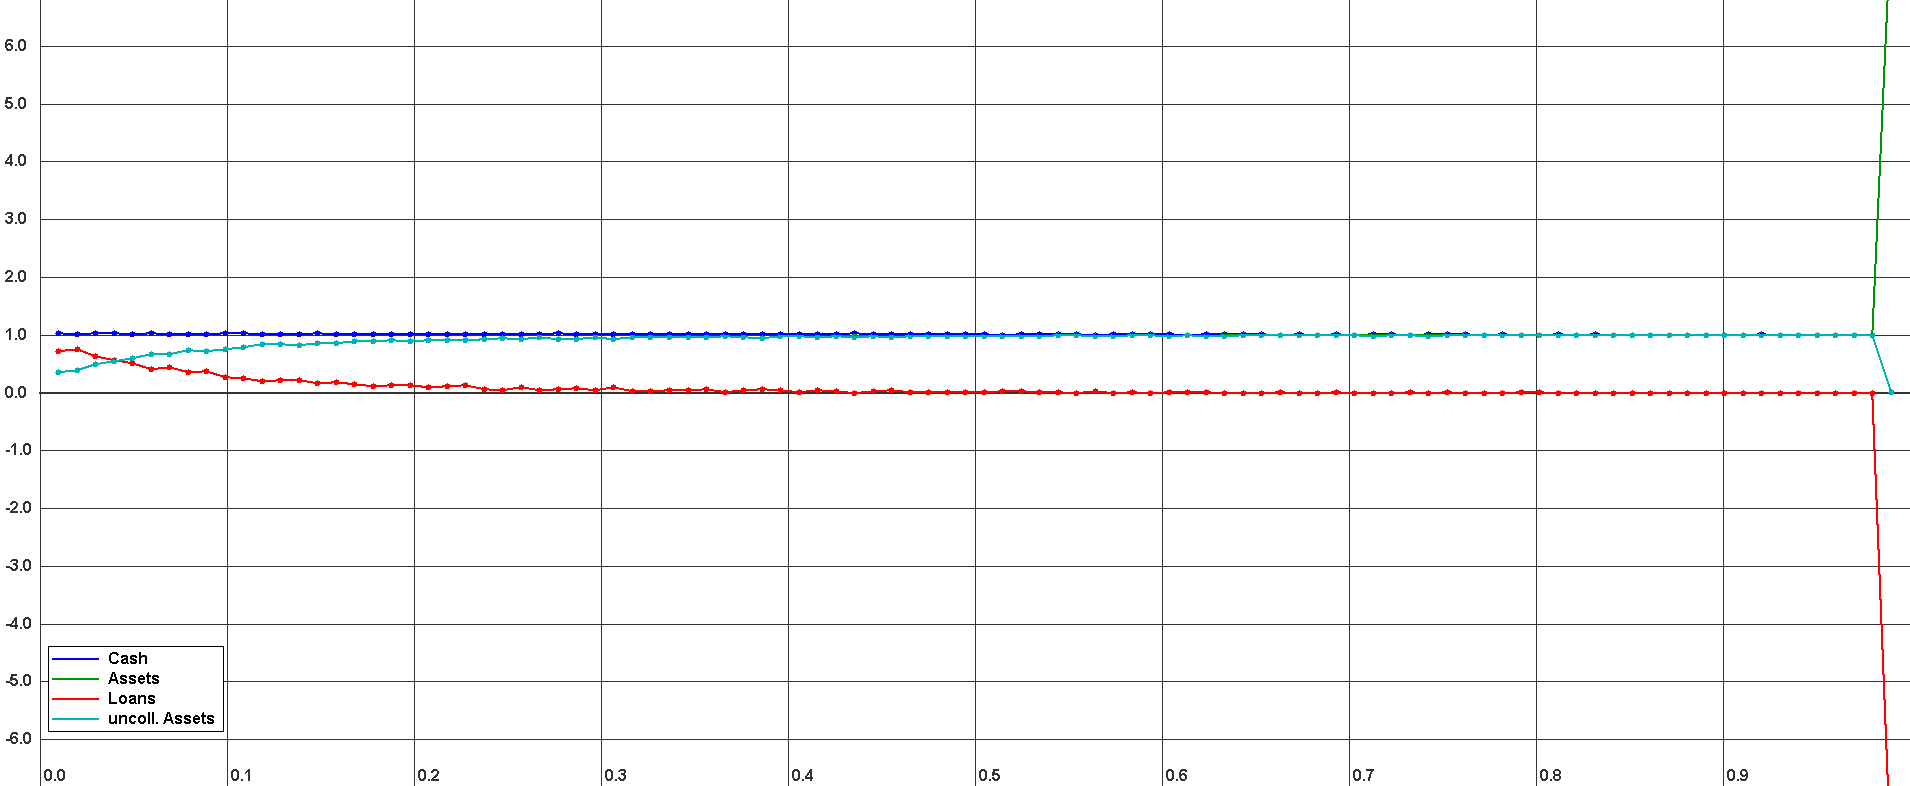
\includegraphics[width=1.0\textwidth, angle=0]{MAXIMUMHUB_100_NOCOLLATERALMARKET_REPL.png}
	\caption{Wealth-Distribution of Maximum-Hub topology}
	\label{fig:wealth_MAXIMUMHUB_100_NOCOLLATERALMARKET_REPL}
\end{figure}

\section{Scale-Free and Small-World topologies}
This topologies fail to come even close to equilibrium too due to reasons given in chapter \ref{ch:hypothesis} "Hypothesis". This can be seen also very clearly in the visual results and thus no performance- and equilibrium-tables are listed as they would not make any sense.

\subsection{Erdos-Renyi}
Note that with the correct parametrization this topology could satisfy the hypothesis by pure chance. The result would be a pure random network as an Ascending-Connected topology with random short-cuts but as already showed above this Ascending-Connected random short-cuts network fails from producing the theoretical and Fully-Connected equilibrium.

\begin{figure}[H]
	\centering
  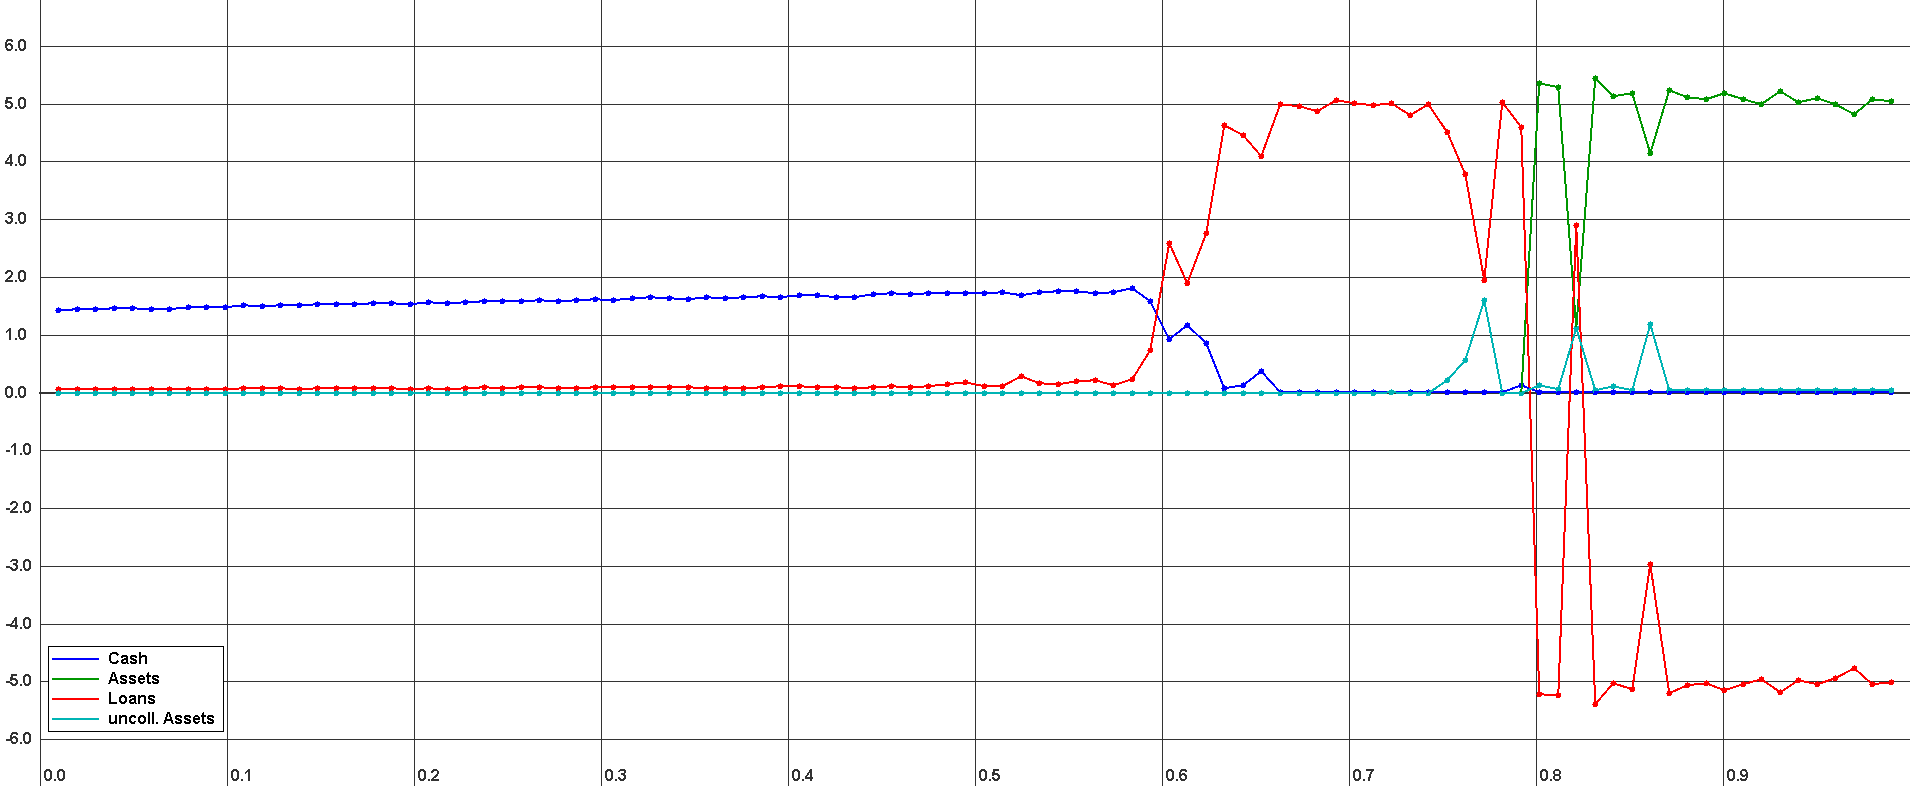
\includegraphics[width=1.0\textwidth, angle=0]{ERDOSRENYI_02_100_NOCOLLATERALMARKET_REPL.png}
	\caption{Wealth-Distribution of Erdos-Renyi 0.2 topology}
	\label{fig:wealth_ERDOSRENYI_02_100_NOCOLLATERALMARKET_REPL}
\end{figure}

\begin{figure}[H]
	\centering
  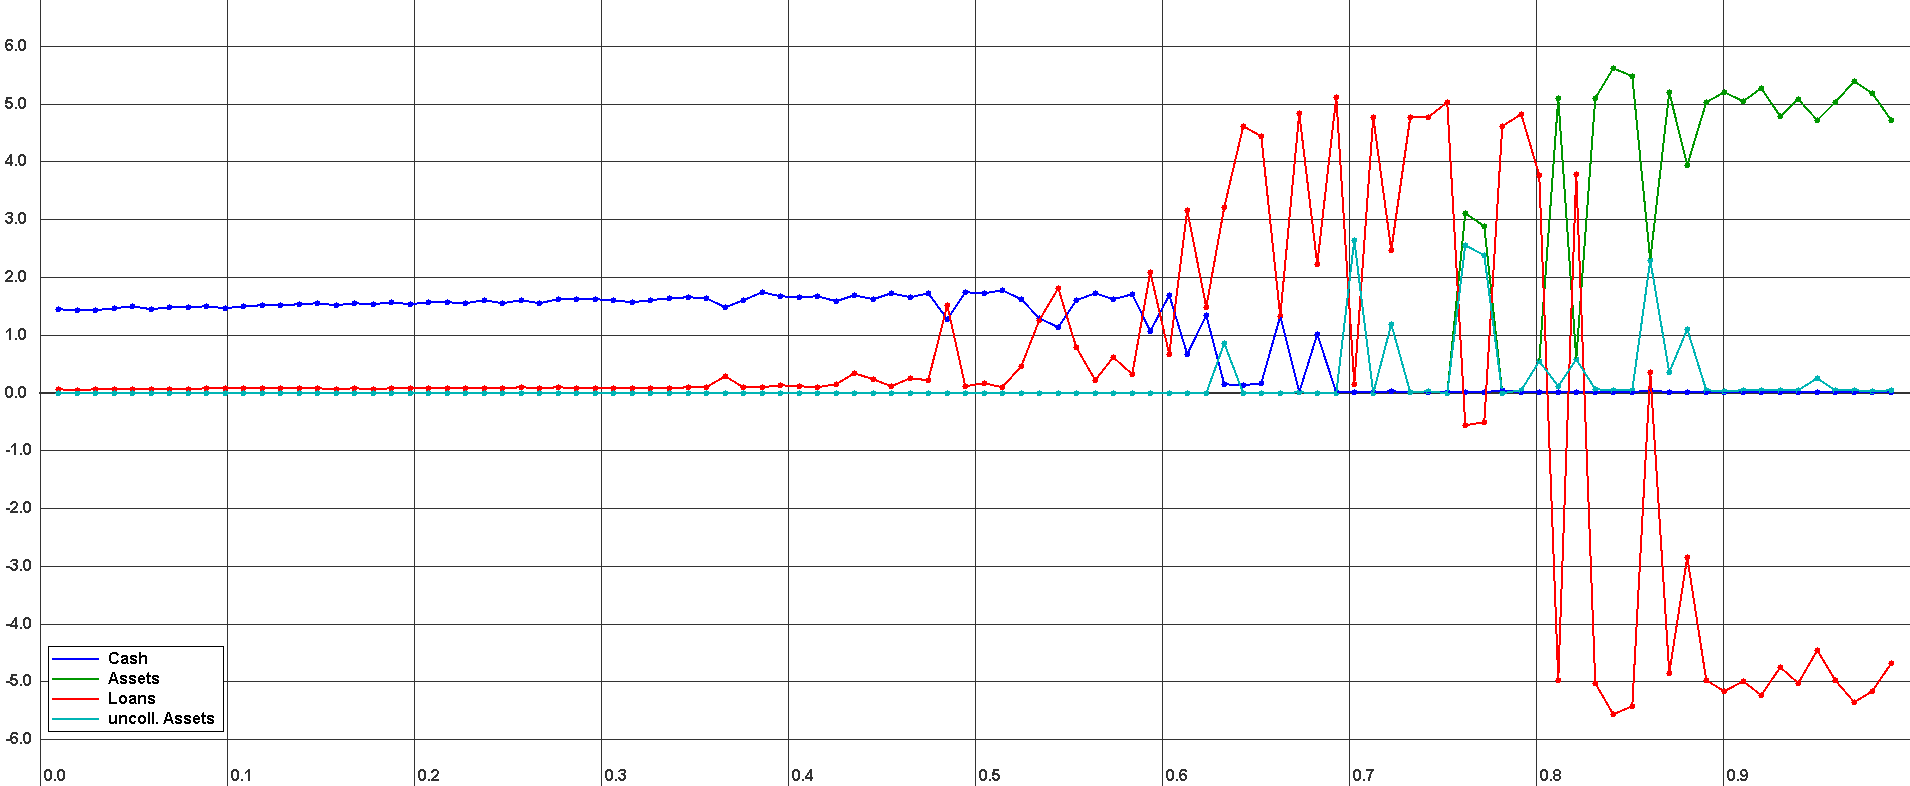
\includegraphics[width=1.0\textwidth, angle=0]{ERDOSRENYI_01_100_NOCOLLATERALMARKET_REPL.png}
	\caption{Wealth-Distribution of Erdos-Renyi 0.1 topology}
	\label{fig:wealth_ERDOSRENYI_01_100_NOCOLLATERALMARKET_REPL}
\end{figure}

\begin{figure}[H]
	\centering
  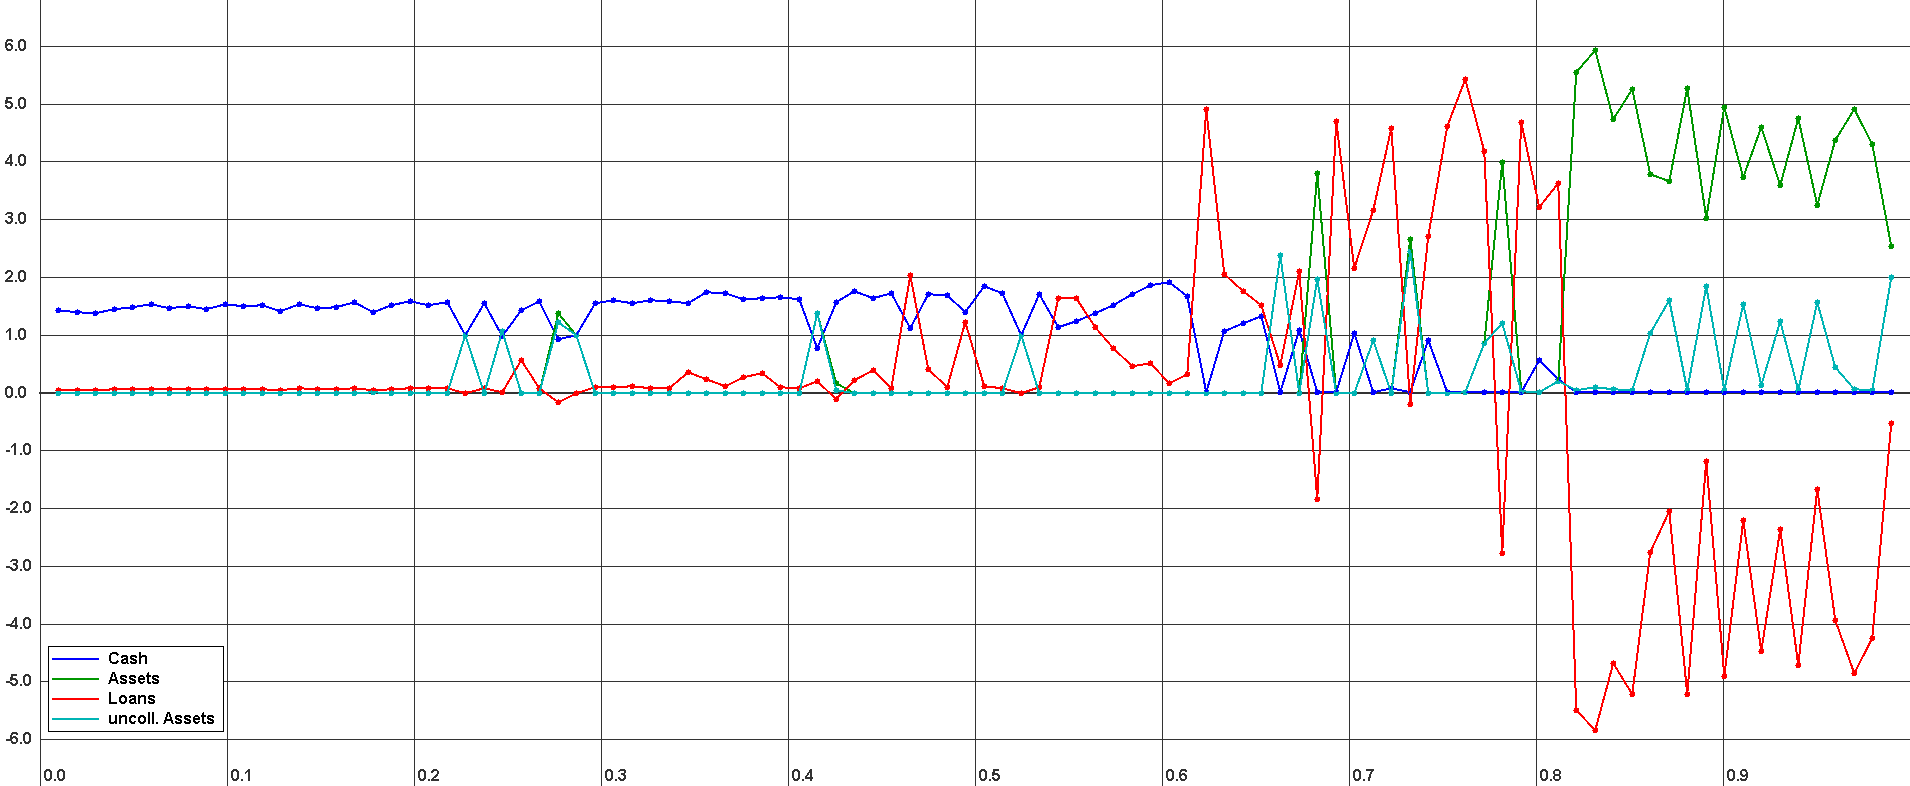
\includegraphics[width=1.0\textwidth, angle=0]{ERDOSRENYI_005_100_NOCOLLATERALMARKET_REPL.png}
	\caption{Wealth-Distribution of Erdos-Renyi 0.05 topology}
	\label{fig:wealth_ERDOSRENYI_005_100_NOCOLLATERALMARKET_REPL}
\end{figure}

\subsection{Barbasi-Albert}
\begin{figure}[H]
	\centering
  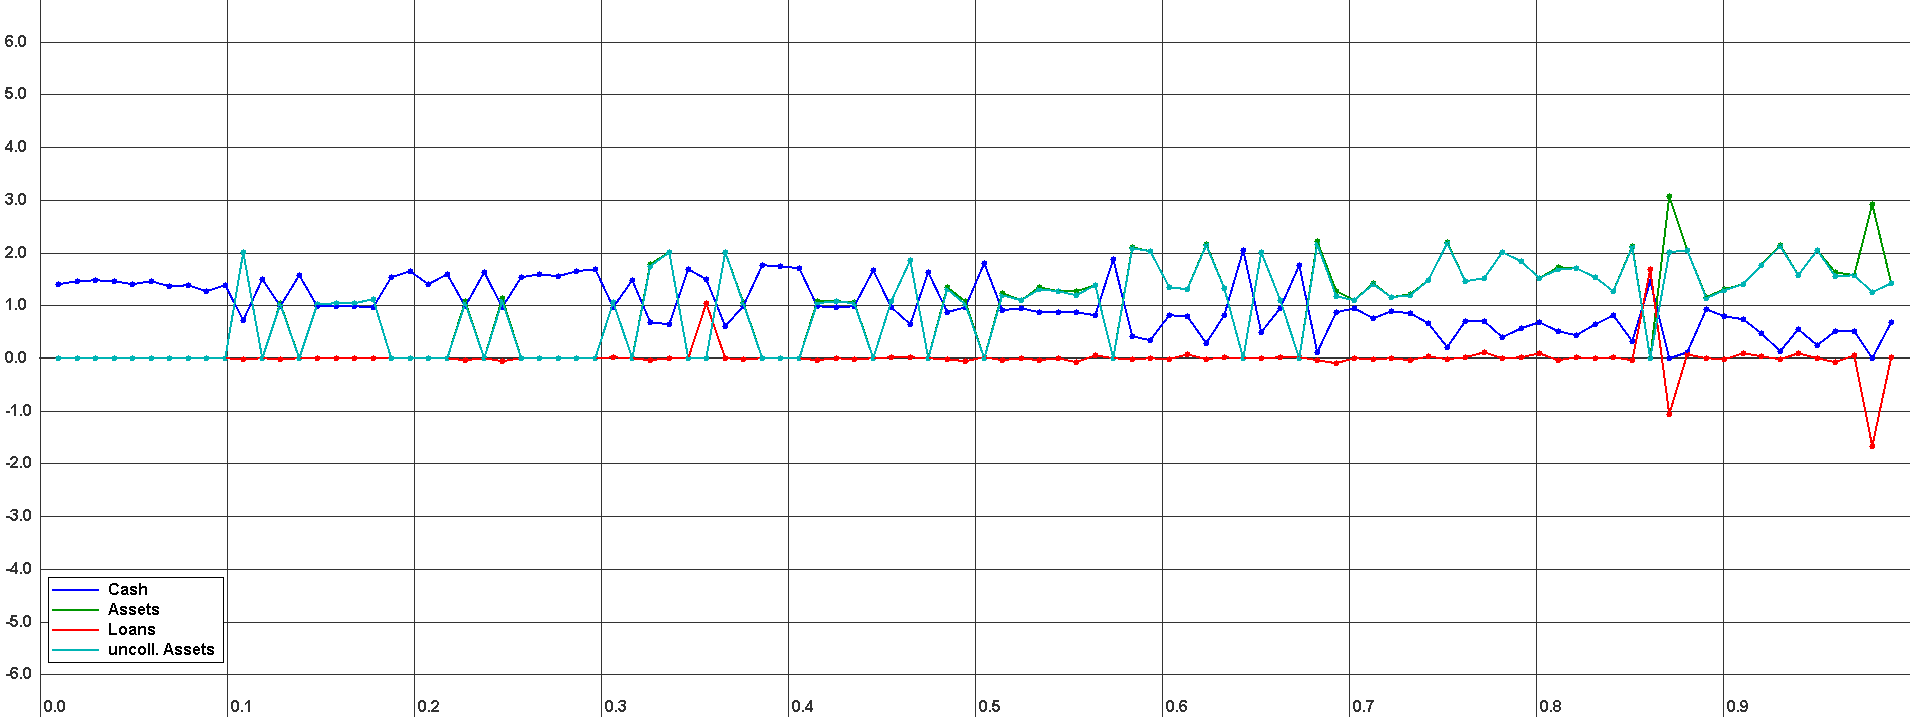
\includegraphics[width=1.0\textwidth, angle=0]{BARBASIALBERT_m03_m1_100_NOCOLLATERALMARKET_REPL.png}
	\caption{Wealth-Distribution of Barbasi-Albert m0=3, m=1 topology}
	\label{fig:wealth_BARBASIALBERT_m03_m1_100_NOCOLLATERALMARKET_REPL}
\end{figure}

\begin{figure}[H]
	\centering
  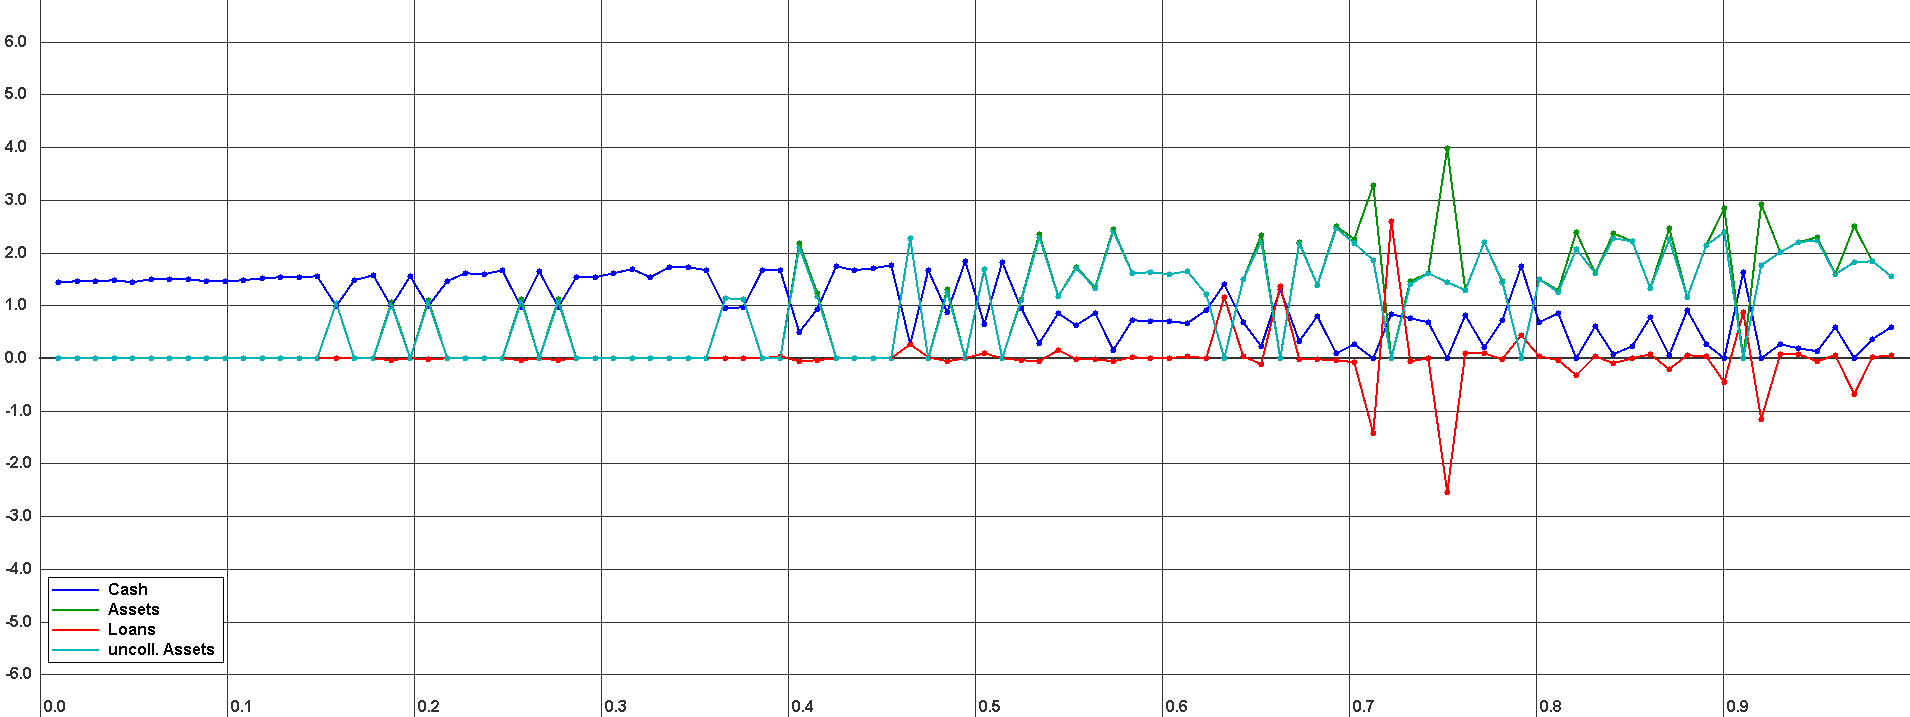
\includegraphics[width=1.0\textwidth, angle=0]{BARBASIALBERT_m09_m3_100_NOCOLLATERALMARKET_REPL.png}
	\caption{Wealth-Distribution of Barbasi-Albert m0=9, m=3 topology}
	\label{fig:wealth_BARBASIALBERT_m09_m3_100_NOCOLLATERALMARKET_REPL}
\end{figure}

\subsection{Watts-Strogatz}
Note that with the correct parametrization this topology could satisfy the hypothesis by pure chance too. The result would be a pure random network as an Ascending-Connected topology with random short-cuts but as already showed above this Ascending-Connected random short-cuts network fails from producing the theoretical and Fully-Connected equilibrium.

\begin{figure}[H]
	\centering
  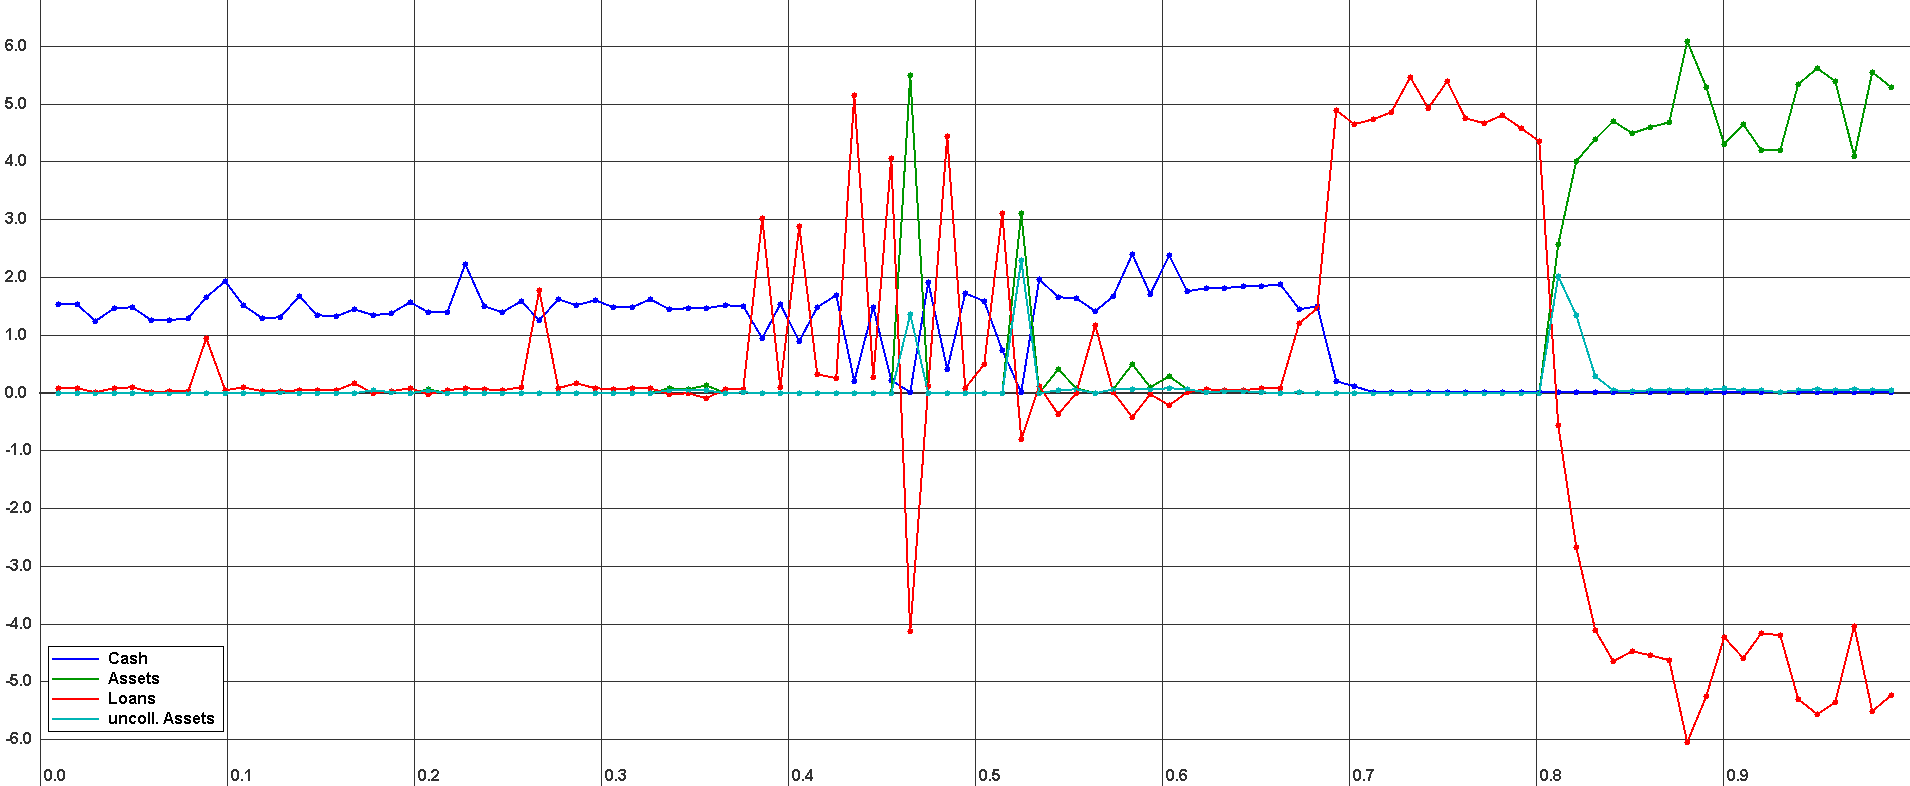
\includegraphics[width=1.0\textwidth, angle=0]{WATTSSTROGATZ_k2_b02_100_NOCOLLATERALMARKET_REPL.png}
	\caption{Wealth-Distribution of Watts-Strogatz k=2, b=0.2 topology}
	\label{fig:wealth_WATTSSTROGATZ_k2_b02_100_NOCOLLATERALMARKET_REPL}
\end{figure}

\begin{figure}[H]
	\centering
  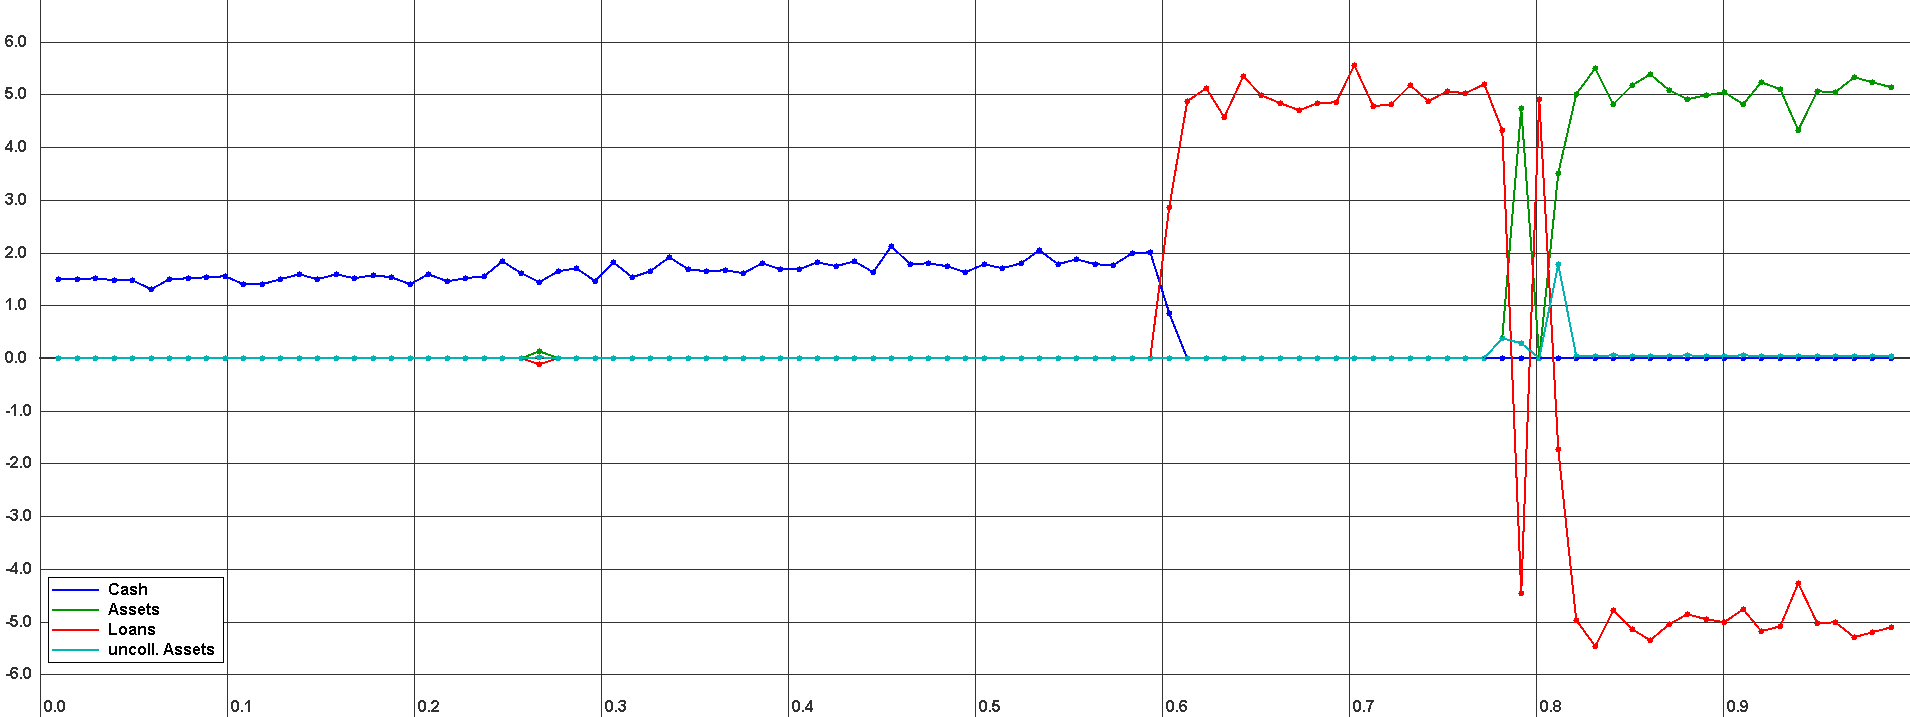
\includegraphics[width=1.0\textwidth, angle=0]{WATTSSTROGATZ_k4_b05_100_NOCOLLATERALMARKET_REPL.png}
	\caption{Wealth-Distribution of Watts-Strogatz k=4, b=0.5 topology}
	\label{fig:wealth_WATTSSTROGATZ_k4_b05_100_NOCOLLATERALMARKET_REPL}
\end{figure}

\end{document}
